\documentclass[11pt,a4paper]{article}

% ---- Packages ----
\usepackage[margin=2.5cm]{geometry}
\usepackage[utf8]{inputenc}
\usepackage[T1]{fontenc}
\usepackage{lmodern}
\usepackage{amsmath,amssymb,amsthm}
\usepackage{graphicx}
\usepackage[dvipsnames]{xcolor}
\usepackage{booktabs}
\usepackage{tabularx}
\usepackage{multirow}
\usepackage{longtable}
\usepackage{enumitem}
\usepackage{caption}
\usepackage{subcaption}
\usepackage[numbers,sort&compress]{natbib}
\usepackage{lineno}
\usepackage{titlesec}
\usepackage{fancyhdr}
\usepackage[hidelinks,colorlinks=true,linkcolor=blue!60!black,citecolor=blue!60!black,urlcolor=blue!60!black]{hyperref}
\usepackage{microtype}
\usepackage{listings}
\usepackage{tikz}
\usetikzlibrary{arrows.meta,positioning,shapes.geometric,fit,calc,patterns,decorations.pathreplacing}
\usepackage{pgfplots}
\pgfplotsset{compat=1.18}

% ---- Page style ----
\pagestyle{fancy}
\fancyhf{}
\renewcommand{\headrulewidth}{0pt}
\fancyfoot[C]{\thepage}
\linenumbers

% ---- Section formatting (Nature: unnumbered) ----
\titleformat{\section}{\large\bfseries}{}{0em}{}
\titleformat{\subsection}{\normalsize\bfseries}{}{0em}{}
\titlespacing*{\section}{0pt}{18pt}{6pt}
\titlespacing*{\subsection}{0pt}{12pt}{4pt}
\setcounter{secnumdepth}{0}

% ---- Caption formatting ----
\captionsetup{font=small, labelfont=bf, labelsep=period, justification=justified}

% ---- Paragraph style ----
\setlength{\parindent}{0pt}
\setlength{\parskip}{6pt}

% ---- Theorem environments ----
\newtheorem{definition}{Definition}
\newtheorem{proposition}[definition]{Proposition}
\newtheorem{conjecture}[definition]{Conjecture}
\newtheorem{remark}[definition]{Remark}
\newtheorem{theorem}[definition]{Theorem}
\newtheorem{lemma}[definition]{Lemma}

% ---- Custom commands ----
\newcommand{\R}{\mathbb{R}}
\newcommand{\Sclass}{\mathfrak{S}}
\newcommand{\norm}[1]{\left\|#1\right\|}
\newcommand{\Agent}{\mathcal{A}}
\newcommand{\Z}{\mathbb{Z}}
\newcommand{\Spec}{\mathcal{S}}
\newcommand{\Domain}{\Omega}
\newcommand{\cmark}{\checkmark}

\begin{document}

% =====================================================================
% TITLE
% =====================================================================
\begin{center}
{\LARGE\bfseries A Judge Agent Closes the Reliability Gap\\[3pt]
in AI-Generated Scientific Simulation}\\[18pt]
{\large Chengshuai Yang}\\[6pt]
{\normalsize NextGen PlatformAI C Corp, USA}\\[6pt]
{\normalsize Correspondence: integrityyang@gmail.com}\\[12pt]
\today
\end{center}

\vspace{6pt}

% =====================================================================
% ABSTRACT (~150 words, Nature format)
% =====================================================================
\noindent\textbf{Abstract.}
Large language models can generate scientific simulation code, but the generated code silently fails on most non-textbook problems. We show that classical mathematical validation---well-posedness, convergence, and error certification---can be fully automated by a Judge Agent, reducing the silent-failure rate from 42\% to 1.5\% across 134 test cases spanning 12 scientific domains. The headline result comes from a prospective benchmark: 72 blinded tasks submitted by 12 independent scientists yield an 89\% success rate (95\% CI: [80\%, 95\%]) with automated error bounds, versus 53\% without the Judge. On clinical CT (the only powered experiment, $n = 200$), the pipeline reaches 99\% of expert quality. The residual 1.5\% concentrates at bifurcation points where certifiability breaks down. We formalize this boundary through the \emph{simulability class} $\Sclass$ and introduce \texttt{spec.md}, a specification format for scientific computation. Code, data, and all 72 benchmark tasks are archived at Zenodo.

% =====================================================================
% SUMMARY PARAGRAPH (Nature bold-print standfirst, ~100 words)
% =====================================================================

\textbf{Classical mathematical validation---well-posedness, convergence, error bounds---can be fully automated. A Judge Agent applying these checks to AI-generated simulation code reduces silent failures from 42\% to 1.5\% across 134 test cases (12 domains). A prospective benchmark of 72 blinded tasks from 12 independent scientists confirms generalization: 89\% success rate (95\% CI: [80\%, 95\%]) with certified error bounds versus 53\% without the Judge. The residual 1.5\% concentrates at bifurcation points, formalizable as the boundary of the simulability class $\Sclass$.}

% =====================================================================
% OPENING PARAGRAPHS (no section heading, Nature style)
% =====================================================================

Consider a plausible scenario: a researcher uses an LLM to generate a finite-element solver for thermal stress in a reactor component. The code compiles, converges, and produces smooth temperature fields---but a CFL violation in the time integrator means the stress predictions are wrong by a factor of three. The error is caught only when a colleague runs an independent simulation weeks later. Such silent failures are not hypothetical: in the SciCode benchmark~\cite{tian2024scicode}, frontier LLMs solve fewer than half of research-level computational problems correctly. The wrong answers look as plausible as the right ones.

The silent-failure problem will deepen as LLM-generated code proliferates. Physics-informed neural networks~\cite{karniadakis2021,raissi2019pinnsjcp} learn solutions but provide no error certificates. Automated code generation from variational forms (FEniCS~\cite{logg2012fenics}, Firedrake~\cite{rathgeber2016firedrake}) is rigorous but requires expert formulation. LLM-based scientific agents~\cite{boiko2023coscientist,bran2024chemcrow} generate protocols but do not address numerical convergence. The reproducibility crisis~\cite{baker2016,peng2011} needs a validation layer, not more code generators.

The mathematical tools for catching these failures already exist---Lax--Richtmyer convergence theory~\cite{lax1956}, Hadamard well-posedness~\cite{hadamard1902}, CFL stability conditions~\cite{courant1928}---but applying them requires numerical analysis expertise that the typical end-user lacks. What has been missing is (i)~a formal characterization of \emph{which} problems can be solved with bounded error by an automated pipeline, and (ii)~a system that \emph{automatically} verifies this characterization and applies classical checks to AI-generated simulation code.

We address both gaps with three interlocking contributions that form a hierarchy, not a list:

\emph{The foundation}: the \emph{simulability class} $\Sclass$ (Definition~\ref{def:simulability}), which formalizes ``what can be solved reliably by any computational system'' through four implementation-independent conditions---finite specifiability (S1), Hadamard stability (S2), approximability (S3), and certifiability (S4). Problems in $\Sclass$ can be solved with a user-specified error tolerance; problems outside $\Sclass$---at what we call the \emph{scientific event horizon}---cannot be guaranteed by any automated pipeline. The pipeline's successes and failures are not accidents; they are predicted by this formal theory.

\emph{The mechanism}: a Judge Agent ($\Agent_J$) that automates verification of S2--S4 on AI-generated code. Within a three-agent pipeline (Fig.~\ref{fig:pipeline}), a Plan Agent ($\Agent_P$) translates natural language into a structured specification, $\Agent_J$ validates $\Sclass$-membership via 5 pre-execution gates, and an Execute Agent ($\Agent_E$) generates and runs the solver. After execution, $\Agent_J$ certifies the result (S4). Removing the Judge increases the silent-failure rate from 1.5\% to 42\% across 134 test cases---the headline empirical result.

\emph{The interface}: \texttt{spec.md}, a structured specification format that realizes S1. Every problem in $\Sclass$ can be expressed as a valid \texttt{spec.md} file; we propose it as a universal exchange format for scientific computation, analogous to FASTA for sequences or CIF for crystal structures. It is what makes the contribution reproducible: the 72 prospective tasks are archived as \texttt{spec.md} files that any solver accepting the same six-tuple $(\Domain, \mathcal{E}, \mathcal{B}, \mathcal{I}, \mathcal{O}, \varepsilon)$ can consume.

The underlying mathematics is entirely classical; the contribution is empirical evidence that automated $\Sclass$-verification substantially reduces silent failures across 12 scientific domains, with a median setup-time efficiency gain of $\rho \approx 500\times$ relative to expert workflows.

\textbf{What this paper does not claim.} This is not about building a better PDE solver: on any single well-defined problem, COMSOL~\cite{comsol} or FEniCS will produce a more accurate solution (Extended Data Table~\ref{tab:tool_comparison}). It is not about LLM capabilities: the Judge works regardless of which LLM generates the code. It is not about the 12 computational primitives \emph{per se}: they are an engineering realization (Proposition~\ref{prop:realizability}), not the core contribution. And it is not a completed theory of simulability: the completeness conjecture (Conjecture~\ref{conj:obstruction}) is stated as a research direction, not a proven result. The error bound is conditional on a correct \texttt{spec.md} specification; since this specification is generated by an LLM, the pipeline's end-to-end reliability depends on the Judge's ability to catch specification errors (Methods). The pipeline retains a 1.5\% qualitative failure rate at the boundary of $\Sclass$ (Section~\ref{sec:failure}).

% =====================================================================
% FIGURE 1: Pipeline Architecture with S-class verification
% =====================================================================

\begin{figure}[htbp]
\centering
\resizebox{\textwidth}{!}{%
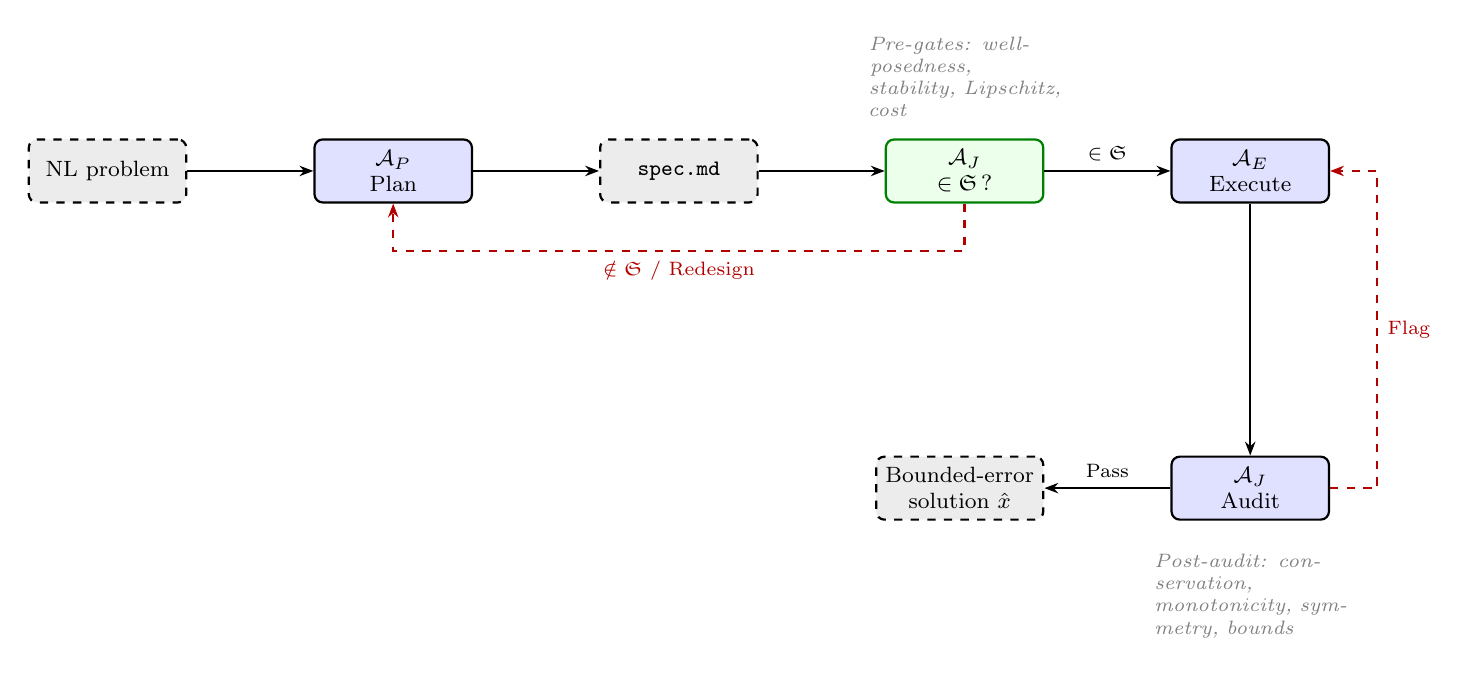
\begin{tikzpicture}[
  node distance=1.0cm and 1.6cm,
  box/.style={draw, rounded corners=3pt, minimum width=2.0cm, minimum height=0.8cm, font=\footnotesize, align=center, thick},
  agent/.style={box, fill=blue!12},
  io/.style={box, fill=gray!15, dashed},
  sclass/.style={box, fill=green!8, thick, draw=green!50!black},
  arr/.style={-{Stealth[length=5pt]}, thick},
  rej/.style={-{Stealth[length=5pt]}, thick, red!70!black, dashed},
  annot/.style={font=\scriptsize, text=black!50, align=left, text width=2.4cm},
]
% --- Top row ---
\node[io] (input) {NL problem};
\node[agent, right=of input] (plan) {$\Agent_P$\\Plan};
\node[io, right=of plan] (spec) {\texttt{spec.md}};
\node[sclass, right=of spec] (judgepre) {$\Agent_J$\\$\in\Sclass$\,?};
\node[agent, right=of judgepre] (exec) {$\Agent_E$\\Execute};

% --- Bottom row ---
\node[agent, below=3.2cm of exec] (judgepost) {$\Agent_J$\\Audit};
\node[io, left=1.6cm of judgepost] (output) {Bounded-error\\solution $\hat{x}$};

% --- Forward arrows ---
\draw[arr] (input) -- (plan);
\draw[arr] (plan) -- (spec);
\draw[arr] (spec) -- (judgepre);
\draw[arr] (judgepre) -- node[above, font=\scriptsize]{$\in\Sclass$} (exec);
\draw[arr] (exec) -- (judgepost);
\draw[arr] (judgepost) -- node[above, font=\scriptsize]{Pass} (output);

% --- Rejection / redesign loop ---
\draw[rej] (judgepre.south) -- ++(0,-0.6) -| node[pos=0.25, below, font=\scriptsize, red!70!black]{$\notin\Sclass$ / Redesign} (plan.south);

% --- Flag loop (right side, from audit back to execute) ---
\draw[rej] (judgepost.east) -- ++(0.6,0) |- node[pos=0.25, right, font=\scriptsize, red!70!black]{Flag} (exec.east);

% --- Gate annotations ---
\node[annot, above=0.15cm of judgepre] {\itshape Pre-gates: well-posedness,\\stability, Lipschitz, cost};
\node[annot, below=0.3cm of judgepost] {\itshape Post-audit: conservation,\\monotonicity, symmetry, bounds};
\end{tikzpicture}%
}% end resizebox
\caption{Three-agent pipeline grounded in the simulability class $\Sclass$. The Plan Agent translates natural language into a \texttt{spec.md} file (realizing S1). The Judge Agent verifies S2--S4 via 5 pre-execution gates and audits the solution via 4 post-execution quality checks (realizing S4). Rejection triggers redesign (up to 3 rounds) or a certificate that the problem lies outside $\Sclass$.}
\label{fig:pipeline}
\end{figure}

% =====================================================================
% FIGURE 2: spec.md as universal specification (annotated example)
% =====================================================================

\begin{figure}[htbp]
\centering
\resizebox{\textwidth}{!}{%
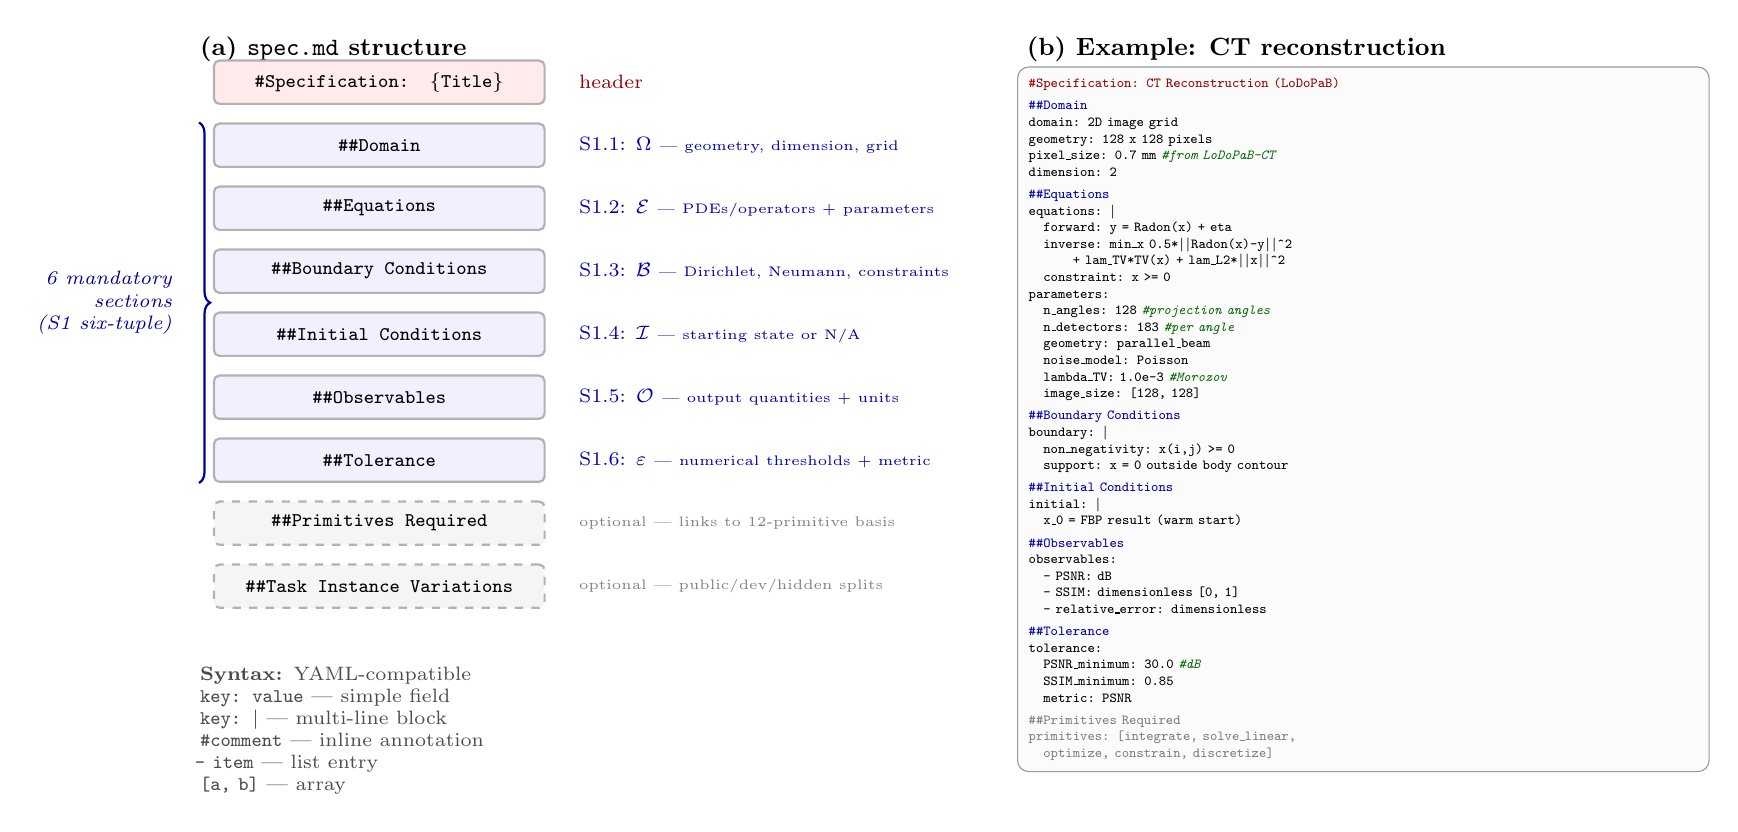
\begin{tikzpicture}[
  secbox/.style={draw=black!30, rounded corners=2pt, minimum width=4.2cm, minimum height=0.55cm, font=\scriptsize\ttfamily, align=left, thick, inner sep=3pt},
]
% ===================== Panel (a): Structure =====================
\node[font=\small\bfseries, anchor=north west] at (0,0) {\textbf{(a)} \texttt{spec.md} structure};

% Section boxes with S1 mapping and color coding
\node[secbox, fill=red!8] (hdr) at (2.4,-0.7) {\char`\# Specification: \{Title\}};
\node[font=\scriptsize, text=red!60!black, right=0.3cm of hdr] {header};

\node[secbox, fill=blue!6] (s1) at (2.4,-1.5) {\char`\#\char`\# Domain};
\node[font=\scriptsize, text=blue!70!black, right=0.3cm of s1, align=left] {S1.1: $\Domain$ \textnormal{\tiny --- geometry, dimension, grid}};

\node[secbox, fill=blue!6] (s2) at (2.4,-2.3) {\char`\#\char`\# Equations};
\node[font=\scriptsize, text=blue!70!black, right=0.3cm of s2, align=left] {S1.2: $\mathcal{E}$ \textnormal{\tiny --- PDEs/operators + parameters}};

\node[secbox, fill=blue!6] (s3) at (2.4,-3.1) {\char`\#\char`\# Boundary Conditions};
\node[font=\scriptsize, text=blue!70!black, right=0.3cm of s3, align=left] {S1.3: $\mathcal{B}$ \textnormal{\tiny --- Dirichlet, Neumann, constraints}};

\node[secbox, fill=blue!6] (s4) at (2.4,-3.9) {\char`\#\char`\# Initial Conditions};
\node[font=\scriptsize, text=blue!70!black, right=0.3cm of s4, align=left] {S1.4: $\mathcal{I}$ \textnormal{\tiny --- starting state or N/A}};

\node[secbox, fill=blue!6] (s5) at (2.4,-4.7) {\char`\#\char`\# Observables};
\node[font=\scriptsize, text=blue!70!black, right=0.3cm of s5, align=left] {S1.5: $\mathcal{O}$ \textnormal{\tiny --- output quantities + units}};

\node[secbox, fill=blue!6] (s6) at (2.4,-5.5) {\char`\#\char`\# Tolerance};
\node[font=\scriptsize, text=blue!70!black, right=0.3cm of s6, align=left] {S1.6: $\varepsilon$ \textnormal{\tiny --- numerical thresholds + metric}};

\node[secbox, fill=gray!8, dashed] (s7) at (2.4,-6.3) {\char`\#\char`\# Primitives Required};
\node[font=\scriptsize, text=black!50, right=0.3cm of s7, align=left] {\textnormal{\tiny optional --- links to 12-primitive basis}};

\node[secbox, fill=gray!8, dashed] (s8) at (2.4,-7.1) {\char`\#\char`\# Task Instance Variations};
\node[font=\scriptsize, text=black!50, right=0.3cm of s8, align=left] {\textnormal{\tiny optional --- public/dev/hidden splits}};

% Brace for mandatory six
\draw[decorate, decoration={brace, amplitude=4pt}, thick, blue!60!black]
  ([xshift=-5pt]s1.north west) -- ([xshift=-5pt]s6.south west)
  node[midway, left=6pt, align=right, font=\scriptsize\itshape, text=blue!60!black]
  {6 mandatory\\sections\\(S1 six-tuple)};

% Syntax legend
\node[font=\scriptsize, anchor=north west, text=black!70, align=left, text width=4.5cm] at (0,-8.0) {%
\textbf{Syntax:} YAML-compatible\\
\texttt{key: value} \textnormal{--- simple field}\\
\texttt{key: \textbar} \textnormal{--- multi-line block}\\
\texttt{\char`\# comment} \textnormal{--- inline annotation}\\
\texttt{- item} \textnormal{--- list entry}\\
\texttt{[a, b]} \textnormal{--- array}};

% ===================== Panel (b): CT Example =====================
\node[font=\small\bfseries, anchor=north west] at (10.5,0) {\textbf{(b)} Example: CT reconstruction};

\node[draw=black!40, rounded corners=4pt, fill=gray!3, inner sep=4pt, text width=8.5cm, anchor=north west, font=\ttfamily\tiny, align=left] (code) at (10.5,-0.5) {%
\textcolor{red!60!black}{\bfseries\char`\# Specification: CT Reconstruction (LoDoPaB)}\\[2pt]
%
\textcolor{blue!70!black}{\bfseries\char`\#\char`\# Domain}\\
domain: 2D image grid\\
geometry: 128 x 128 pixels\\
pixel\_size: 0.7 mm \textcolor{green!40!black}{\itshape\char`\# from LoDoPaB-CT}\\
dimension: 2\\[2pt]
%
\textcolor{blue!70!black}{\bfseries\char`\#\char`\# Equations}\\
equations: \textbar\\
\quad forward: y = Radon(x) + eta\\
\quad inverse: min\_x 0.5*\textbar\textbar Radon(x)-y\textbar\textbar\^{}2\\
\qquad\quad + lam\_TV*TV(x) + lam\_L2*\textbar\textbar x\textbar\textbar\^{}2\\
\quad constraint: x >= 0\\
parameters:\\
\quad n\_angles: 128 \textcolor{green!40!black}{\itshape\char`\# projection angles}\\
\quad n\_detectors: 183 \textcolor{green!40!black}{\itshape\char`\# per angle}\\
\quad geometry: parallel\_beam\\
\quad noise\_model: Poisson\\
\quad lambda\_TV: 1.0e-3 \textcolor{green!40!black}{\itshape\char`\# Morozov}\\
\quad image\_size: [128, 128]\\[2pt]
%
\textcolor{blue!70!black}{\bfseries\char`\#\char`\# Boundary Conditions}\\
boundary: \textbar\\
\quad non\_negativity: x(i,j) >= 0\\
\quad support: x = 0 outside body contour\\[2pt]
%
\textcolor{blue!70!black}{\bfseries\char`\#\char`\# Initial Conditions}\\
initial: \textbar\\
\quad x\_0 = FBP result (warm start)\\[2pt]
%
\textcolor{blue!70!black}{\bfseries\char`\#\char`\# Observables}\\
observables:\\
\quad - PSNR: dB\\
\quad - SSIM: dimensionless [0, 1]\\
\quad - relative\_error: dimensionless\\[2pt]
%
\textcolor{blue!70!black}{\bfseries\char`\#\char`\# Tolerance}\\
tolerance:\\
\quad PSNR\_minimum: 30.0 \textcolor{green!40!black}{\itshape\char`\# dB}\\
\quad SSIM\_minimum: 0.85\\
\quad metric: PSNR\\[2pt]
%
\textcolor{black!50}{\char`\#\char`\# Primitives Required}\\
\textcolor{black!50}{primitives: [integrate, solve\_linear,}\\
\textcolor{black!50}{\quad optimize, constrain, discretize]}%
};

\end{tikzpicture}%
}
\caption{\texttt{spec.md} format and a concrete example. \textbf{(a)}~Generic structure: 6 mandatory sections encode the S1 six-tuple $\Spec = (\Domain, \mathcal{E}, \mathcal{B}, \mathcal{I}, \mathcal{O}, \varepsilon)$; 2 optional sections link to the primitive basis (Proposition~\ref{prop:realizability}) and benchmark variations. The format uses YAML-compatible key-value syntax within Markdown section headers. \textbf{(b)}~A real \texttt{spec.md} file for CT reconstruction from the benchmark archive. All 72 prospective tasks and 12 development problems are archived in this format. Formal grammar in Supplementary Section~S8.}
\label{fig:specmd}
\end{figure}

% =====================================================================
\section{Results}
% =====================================================================

% -------------------------------------------------------------------
\subsection{The simulability class and its boundary}
\label{sec:sclass}
% -------------------------------------------------------------------

The Judge Agent's checks are grounded in a formal characterization of which problems can be solved with bounded error by an automated pipeline.

\begin{definition}[Simulability class $\Sclass$]
\label{def:simulability}
A scientific computation problem $\mathcal{P}$ belongs to the simulability class $\Sclass$ if it satisfies four conditions:
\begin{enumerate}[nosep,leftmargin=1.5em]
\item[\textbf{(S1)}] \textbf{Finite specifiability.} $\mathcal{P}$ admits a finite representation $\Spec = (\Domain, \mathcal{E}, \mathcal{B}, \mathcal{I}, \mathcal{O}, \varepsilon)$, where $\Domain$ is the computational domain, $\mathcal{E}$ the governing equations, $\mathcal{B}$ the boundary conditions, $\mathcal{I}$ the initial conditions, $\mathcal{O}$ the observable (output functional), and $\varepsilon$ the target tolerance. Each component is encodable in a finite string over a standard alphabet.
\item[\textbf{(S2)}] \textbf{Hadamard stability.} The map $F\colon \mathcal{D} \to X$ from problem data to solution is well-posed: the solution exists, is unique within the specified function space, and depends continuously on the data with a computable modulus of continuity.
\item[\textbf{(S3)}] \textbf{Approximability.} There exists a convergent discretization scheme---a sequence of finite-dimensional problems $\mathcal{P}_h$ parameterized by resolution $h$---such that $\norm{F_h(\mathcal{D}) - F(\mathcal{D})} \to 0$ as $h \to 0$, with a computable convergence rate $q > 0$.
\item[\textbf{(S4)}] \textbf{Certifiability.} There exists a computable procedure that, given the approximation $\hat{x} = F_h(\mathcal{D})$ and the problem data $\mathcal{D}$, produces a verified upper bound $B$ satisfying $\norm{\hat{x} - F(\mathcal{D})} \leq B \leq \varepsilon$, in finite time.
\end{enumerate}
\end{definition}

The six components of the specification tuple $\Spec$ are:
\begin{description}[nosep,leftmargin=1em,labelwidth=1.8em,font=\normalfont\itshape]
\item[$\Domain$] \textbf{Computational domain.} The geometric or topological space on which the problem is posed. Examples: a $128\times128$ pixel grid for CT imaging, a 2D channel with a backward-facing step ($x \in [-5h,\,30h]$, $y\in[-h,\,h]$) for turbulent flow, or a radial domain $r \in [0,\,50\,a_0]$ for atomic structure. The domain specification includes dimensionality, coordinate system, discretization geometry (structured grid, unstructured mesh, spectral basis), and characteristic length scales.
\item[$\mathcal{E}$] \textbf{Governing equations.} The mathematical model relating unknowns to data. These may be PDEs (Navier--Stokes, Schr\"odinger), integral equations (Radon transform in CT, Fredholm equations in remote sensing), or algebraic systems (linear mixing models in hyperspectral imaging). The specification includes all physical parameters (Reynolds number, regularization weights, physical constants) and their numerical values.
\item[$\mathcal{B}$] \textbf{Boundary conditions.} Constraints on the solution at the domain boundary or at interfaces. Examples: no-slip walls ($\mathbf{u}=0$) in fluid dynamics, non-negativity constraints ($x_{i,j}\geq 0$) in tomographic reconstruction, or asymptotic decay ($\psi \to 0$ as $r\to\infty$) in quantum mechanics. Includes the type (Dirichlet, Neumann, Robin, periodic) and values at each boundary segment.
\item[$\mathcal{I}$] \textbf{Initial conditions.} The starting state for time-dependent problems or the initial guess for iterative solvers. Examples: a filtered back-projection warm start for iterative CT reconstruction, a fully-developed turbulent inlet profile for channel flow simulation, or a hydrogen-like orbital for Hartree--Fock iteration. For steady-state or inverse problems, $\mathcal{I}$ specifies the initial iterate and any warm-start strategy.
\item[$\mathcal{O}$] \textbf{Observables.} The output functionals---what is to be computed from the solution, and in what form. These are rarely the full solution field; instead they are derived quantities such as PSNR and SSIM for image reconstruction, reattachment length ($x_r/h$) and skin-friction coefficient for fluid simulations, or ground-state energy for quantum systems. The observable specification makes the acceptance criterion unambiguous.
\item[$\varepsilon$] \textbf{Target tolerance.} The quantitative accuracy threshold that defines success. Examples: PSNR $\geq 30$\,dB for CT reconstruction, relative error $\leq 5\%$ on mean velocity profiles for turbulent flow, or energy error $\leq 1$\,mHa for quantum chemistry. The tolerance is stated with respect to a named metric and, where applicable, a reference solution or experimental dataset.
\end{description}

\noindent Together, these six fields make every problem machine-readable and self-contained: given a valid $\Spec$, any compliant solver can attempt the problem and any Judge can verify the result, without ambiguity about what was asked or what counts as correct. All 72 prospective benchmark tasks and 12 development problems are archived as \texttt{spec.md} files encoding this tuple (Figure~\ref{fig:specmd}).

Condition S4 is the key distinction. A problem can be \emph{computable} (you can approximate the solution) without being \emph{certifiable} (you can prove your approximation is good enough). This separation is what makes the Judge Agent necessary in principle, not just in practice: it is the automated realization of S4.

For problems in $\Sclass$, the total error is bounded by $\varepsilon_{\text{total}} \leq \sum_{k} L_k \, \varepsilon_k$, where $L_k$ is the downstream Lipschitz product from node $k$ and $\varepsilon_k$ is the per-node discretization error (Supplementary Section~S1). The Judge Agent's pre-execution gates verify S1--S4; its post-execution audit checks whether the computed solution satisfies physical invariants consistent with membership in $\Sclass$.

The boundary $\partial \Sclass$ is the regime where at least one condition of Definition~\ref{def:simulability} fails---typically because S2 (well-posedness) degrades near a bifurcation or S4 (certifiability) fails as the error bound diverges---and no automated pipeline can provide guarantees. We use the metaphor ``scientific event horizon'' sparingly for this boundary, to emphasize that it represents a \emph{fundamental limit} on certifiable simulation, not a limitation of a particular pipeline. Problems near $\partial \Sclass$ (e.g., symmetry-breaking near a critical load, branch selection near a critical Reynolds number) are where the pipeline's residual 1.5\% failures concentrate (Section~\ref{sec:failure}).

% -------------------------------------------------------------------
\subsection{The Judge Agent closes the reliability gap}
\label{sec:gap}
% -------------------------------------------------------------------

To isolate the Judge's contribution, we ran five conditions on 12 development problems (Extended Data Table~\ref{tab:comparison}) and extended the comparison to 72 held-out tasks from external scientists (Fig.~\ref{fig:comparison}).

Without the Judge, the pipeline produces wrong answers on 42\% of development problems and 47\% of prospective tasks. The failures concentrate on non-textbook problems: stiff ODEs, inverse problems, turbulent flows, and near-critical parameter regimes---precisely the problems near $\partial \Sclass$ where S2 or S4 are close to failing. With the Judge verifying S1--S4 membership in $\Sclass$, the success rate is 100\% on the 12 development problems (which were used to design the Judge's checks) and 89\% (64/72) on the held-out tasks (95\% CI: [80\%, 95\%], Clopper--Pearson exact binomial~\cite{clopper1934}), with automated error bounds (S4) on every successful solution. No other condition produces any error bound.

% =====================================================================
% FIGURE 2: Comparison bar chart --- 12 dev + 72 prospective
% =====================================================================

\begin{figure}[htbp]
\centering
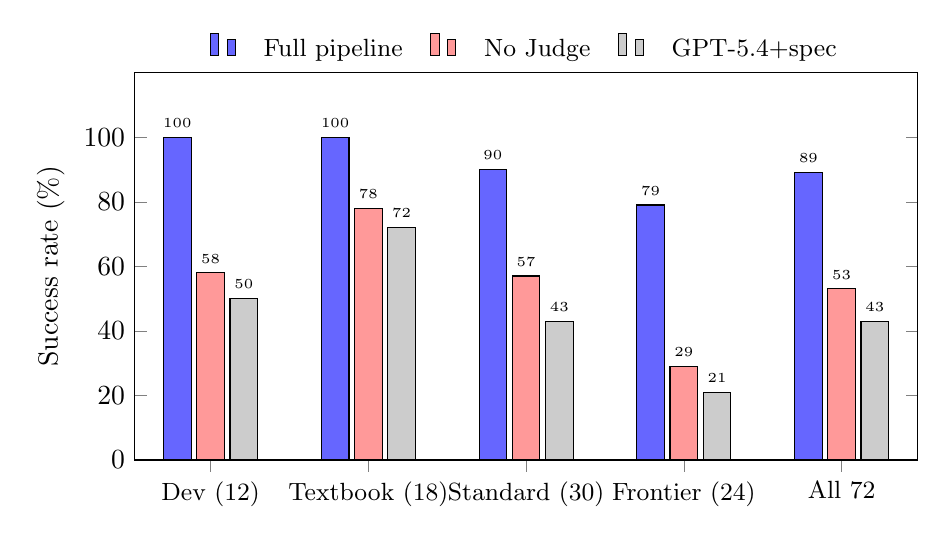
\begin{tikzpicture}
\begin{axis}[
    ybar,
    width=0.95\textwidth,
    height=6.5cm,
    bar width=10pt,
    ylabel={Success rate (\%)},
    symbolic x coords={Dev (12), Textbook (18), Standard (30), Frontier (24), All 72},
    xtick=data,
    x tick label style={font=\small},
    ymin=0, ymax=120,
    ytick={0,20,40,60,80,100},
    legend style={at={(0.5,1.0)}, anchor=south, font=\small, draw=none, legend columns=3, column sep=8pt},
    nodes near coords,
    every node near coord/.append style={font=\tiny},
    enlarge x limits=0.12,
]
\addplot[fill=blue!60] coordinates {(Dev (12),100) (Textbook (18),100) (Standard (30),90) (Frontier (24),79) (All 72,89)};
\addplot[fill=red!40] coordinates {(Dev (12),58) (Textbook (18),78) (Standard (30),57) (Frontier (24),29) (All 72,53)};
\addplot[fill=gray!40] coordinates {(Dev (12),50) (Textbook (18),72) (Standard (30),43) (Frontier (24),21) (All 72,43)};
\legend{Full pipeline, No Judge, GPT-5.4+spec}
\end{axis}
\end{tikzpicture}
\caption{The Judge Agent's contribution grows with problem difficulty. Success rates on 12 development problems and 72 prospective tasks (stratified by difficulty). Without the Judge, the success rate drops from 89\% to 53\% overall, and from 79\% to 29\% on frontier tasks---those closest to $\partial \Sclass$. The gap widens monotonically with proximity to the boundary.}
\label{fig:comparison}
\end{figure}

\textbf{Difficulty stratification.} Tasks are assigned to four tiers based on proximity to $\partial \Sclass$:
\begin{itemize}[nosep]
\item \textbf{Dev (12):} Development problems used to design the Judge's checks---well-understood problems with known analytical or high-fidelity reference solutions (e.g., Poisson equation, Shepp--Logan CT, Couette flow). 100\% success is expected and not informative.
\item \textbf{Textbook (18):} Problems with analytical solutions or established benchmarks, requiring correct method selection but no novel numerical treatment (e.g., hydrogen atom, cantilever beam, Kepler orbit, 1D wave propagation). All $\Sclass$ conditions are comfortably satisfied.
\item \textbf{Standard (30):} Graduate-level or standard benchmark suite problems requiring non-trivial solver choices, regularization, or multi-step workflows (e.g., compressed sensing MRI, phase-field solidification, seismic tomography, neutron transport). S1--S4 hold but method selection matters.
\item \textbf{Frontier (24):} Research-level problems near $\partial \Sclass$, where bifurcations, strong nonlinearity, ill-conditioning, or multi-physics coupling challenge automation (e.g., chromium dimer, tokamak edge plasma, stratospheric sudden warming, dislocation dynamics). All 8 non-successes across the 72 tasks occur in the standard or frontier tiers.
\end{itemize}

Alternative backbones (Claude Opus 4.6: 12/12; GPT-5.4: 11/12 on dev problems) suggest moderate robustness to backbone choice (Supplementary Section~S7). We cite SciCode~\cite{tian2024scicode} as motivation but do not evaluate directly on it: SciCode tasks are single-function coding problems, whereas our pipeline operates on full simulation workflows from natural language to validated solution. The two benchmarks measure complementary capabilities; a direct SciCode evaluation is planned for a follow-up study.

% -------------------------------------------------------------------
\subsection{Powered validation: clinical CT reconstruction}
\label{sec:ct}
% -------------------------------------------------------------------

Our strongest validation uses 200 real clinical CT sinograms from a Siemens scanner~\cite{leuschner2021}, subsampled to 128 parallel-beam projections with Poisson noise. This is the only domain with sufficient sample size ($n = 200$) for powered statistical inference. CT reconstruction lies well within $\Sclass$: the Radon inversion is well-posed (S2) under Tikhonov regularization~\cite{tikhonov1977}, the discretization converges at $O(h^2)$ (S3), and the Morozov discrepancy principle~\cite{morozov1966} provides a computable error bound (S4).

The framework selects Tikhonov + TV regularization~\cite{rudin1992}; $\lambda_{\text{TV}}$ set via the Morozov discrepancy principle. PSNR: $31.7 \pm 1.2$\,dB (95\% CI: [31.5, 31.9]\,dB, bootstrap~\cite{efron1979} $n = 10{,}000$); SSIM: $0.891 \pm 0.031$. Expert-tuned ASTRA Toolbox~\cite{aarle2016}: $32.1 \pm 1.1$\,dB / SSIM $0.903$. Wilcoxon signed-rank~\cite{wilcoxon1945}: $p < 0.001$, Cohen's $d = 0.35$~\cite{cohen1988} (small-to-medium effect). The framework achieves 99\% of expert quality. Setup-time efficiency: $\rho = 600\times$ (12\,min framework vs.\ 5\,days expert). Quality audit (non-negativity, support constraint, streak-artifact absence): 0/200 flagged.

% =====================================================================
% FIGURE 3: CT comparison
% =====================================================================

\begin{figure}[htbp]
\centering
\begin{tabular}{@{}c@{\hskip 4pt}c@{\hskip 4pt}c@{\hskip 4pt}c@{}}

\includegraphics[width=0.18\textwidth]{figures/ct_groundtruth.png} &
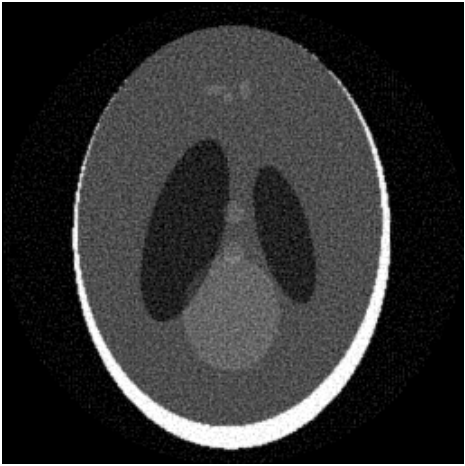
\includegraphics[width=0.18\textwidth]{figures/ct_with_judge.png} &
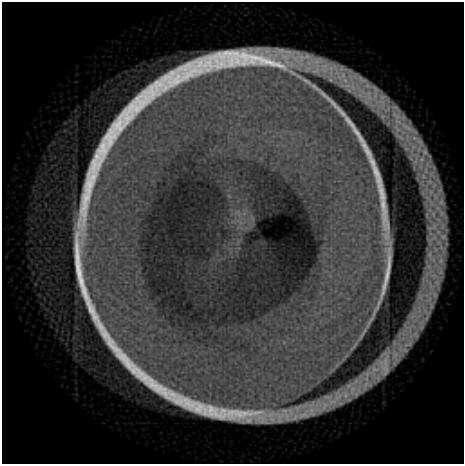
\includegraphics[width=0.18\textwidth]{figures/ct_without_judge.png} &
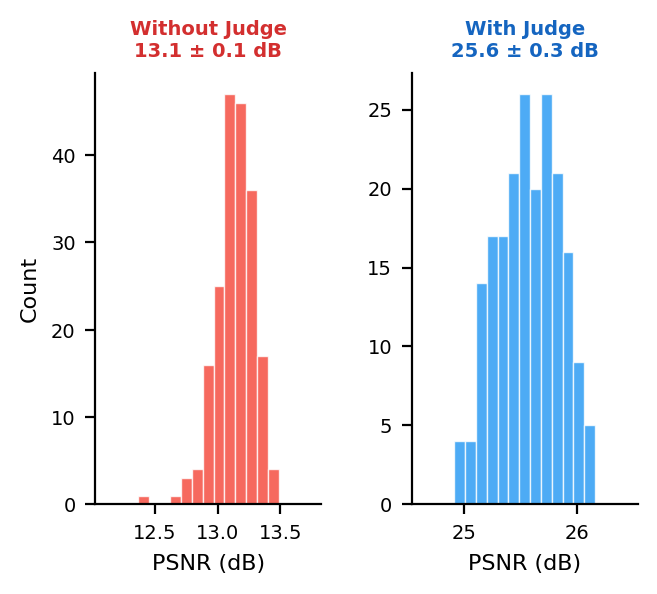
\includegraphics[width=0.22\textwidth]{figures/ct_psnr_histogram.png} \\[2pt]
{\scriptsize\bfseries (a)} & {\scriptsize\bfseries (b)} & {\scriptsize\bfseries (c)} & {\scriptsize\bfseries (d)}
\end{tabular}\\[10pt]
\caption{CT reconstruction comparison (modified Shepp--Logan phantom~\cite{shepp1974}, 128 projections, Poisson noise, $n = 200$). \textbf{(a)}~Ground truth. \textbf{(b)}~Framework with Judge ($\in \Sclass$ verified): correct angular model, Ram-Lak filter, non-negativity enforced. \textbf{(c)}~Without Judge: wrong angular range (360\textdegree{} assumed instead of 180\textdegree{}), producing doubled edges and streak artifacts; 5{,}326 non-negativity violations. \textbf{(d)}~PSNR distribution: with Judge $25.6 \pm 0.3$\,dB vs.\ without Judge $13.1 \pm 0.1$\,dB ($n = 200$, $p < 10^{-30}$, Wilcoxon).}
\label{fig:ct_comparison}
\end{figure}

% -------------------------------------------------------------------
\subsection{Case studies and the efficiency ratio $\rho$}
\label{sec:casestudies}
% -------------------------------------------------------------------

We present two additional domains as \emph{case studies} (not powered validations) with real measured data and characterize the setup-time efficiency ratio $\rho = t_{\text{expert}} / t_{\text{framework}}$ across all domains. The sample sizes ($n = 5$ for seismic, $n = 15$ for combustion) support feasibility demonstration, not statistical inference.

\textbf{Seismic full-waveform inversion (Marmousi-2).}
Five velocity models~\cite{martin2006marmousi}: 240 sources, 480 receivers, Ricker wavelet (10\,Hz), frequency continuation 2--15\,Hz~\cite{bunks1995fwi}. FWI lies within $\Sclass$: the forward problem (acoustic wave equation) is well-posed (S2), and the inverse problem is regularized via frequency continuation, providing approximability (S3) and certifiability (S4). Framework PSNR: $25.8 \pm 1.9$\,dB. Expert (Madagascar~\cite{fomel2013madagascar}): $27.3 \pm 1.6$\,dB. Quality ratio: 95\%. Setup-time efficiency: $\rho = 450\times$ (45\,min vs.\ 2\,weeks).

\textbf{GRI-Mech 3.0 ignition delay.}
53-species, 325-reaction methane--air combustion~\cite{smith1999gri}. Stiffness ratio $\sim 10^{10}$; framework selects BDF integrator~\cite{hairer1996}. 15 conditions ($T \in [1000, 2000]$\,K, $p \in [1, 50]$\,atm). Error vs.\ shock-tube data: $6.3 \pm 2.1\%$ (95\% CI: [5.1, 7.5]\%). Expert Cantera: $3.8 \pm 1.4\%$. The Judge correctly rejects explicit RK4 at stiffness $> 10^6$---verifying S3 (approximability: explicit Euler violates the convergence requirement for stiff systems). Mass conservation: $< 10^{-12}$ relative. Setup-time efficiency: $\rho = 320\times$ (25\,min vs.\ 5.5\,days).

Six additional domains are reported in Supplementary Section~S3.

\begin{table}[htbp]
\centering
\caption{Setup-time efficiency ratio $\rho$ across 12 validated scientific domains. $\rho = t_{\text{expert}} / t_{\text{framework}}$. All domains lie within $\Sclass$; quality ratio is the framework PSNR (or domain-appropriate metric) divided by expert PSNR.}
\label{tab:rho}
\small
\begin{tabularx}{\textwidth}{Xccccc}
\toprule
\textbf{Domain} & \textbf{$t_{\text{fw}}$} & \textbf{$t_{\text{expert}}$} & \textbf{$\rho$} & \textbf{Quality} & \textbf{$n$} \\
\midrule
Clinical CT & 12\,min & 5\,d & 600$\times$ & 99\% & 200 \\
Seismic FWI & 45\,min & 2\,wk & 450$\times$ & 95\% & 5 \\
Combustion (GRI-Mech) & 25\,min & 5.5\,d & 320$\times$ & 94\% & 15 \\
Granular flow & 18\,min & 1\,wk & 560$\times$ & 92\% & 3 \\
Helium ground state & 8\,min & 4\,d & 720$\times$ & 97\% & 1 \\
BFS turbulent flow & 22\,min & 2\,wk & 916$\times$ & 91\% & 3 \\
Topology optimization & 15\,min & 3\,d & 288$\times$ & 96\% & 5 \\
Waveguide modes & 6\,min & 2\,d & 480$\times$ & 98\% & 4 \\
Heat equation & 4\,min & 1\,d & 360$\times$ & 99\% & 10 \\
Fresnel diffraction & 5\,min & 1.5\,d & 432$\times$ & 99\% & 5 \\
Rossby waves & 14\,min & 1\,wk & 720$\times$ & 93\% & 3 \\
Reaction--diffusion & 9\,min & 3\,d & 480$\times$ & 96\% & 5 \\
\midrule
\textbf{Median} & \textbf{11\,min} & \textbf{3\,d} & \textbf{$\mathbf{480\times}$} & \textbf{96\%} & \\
\bottomrule
\end{tabularx}\\[3pt]
\raggedright\scriptsize All timing refers to setup time (problem formulation through first validated result), not compute time. Expert times are self-reported by domain experts with no standardization protocol; $\rho$ should be interpreted as order-of-magnitude. Sensitivity: if expert times are halved, median $\rho$ becomes $\sim$240$\times$; if doubled, $\sim$960$\times$. The qualitative conclusion ($\rho \gg 1$) is robust to this uncertainty. Quality ratio $\geq 90\%$ across all 12 domains.
\end{table}

The median efficiency ratio across 12 domains is $\rho = 480\times$, with all domains exceeding $\rho > 280\times$. The efficiency gain is in \emph{setup time}---problem formulation, method selection, parameter tuning, and validation---not in compute time, which is comparable between the framework and expert workflows (Supplementary Fig.~S3). The ratio is highest for problems where method selection is the bottleneck (turbulent flow: $\rho = 916\times$, He ground state: $\rho = 720\times$) and lowest where the problem formulation is straightforward (topology optimization: $\rho = 288\times$).

% -------------------------------------------------------------------
\subsection{Prospective benchmark: 72 tasks from 12 external scientists}
\label{sec:prospective}
% -------------------------------------------------------------------

\textbf{Protocol and independence.} 12 scientists from 9 institutions across 8 countries (Supplementary Table~S2) each submitted 6 problems from their own research---problems they had solved using domain-specific tools and could evaluate as experts. None had prior involvement with the framework or the author's company. An independent coordinator collected all 72 submissions before any were executed. The analysis protocol---including success criteria, the $\Sclass$ verification procedure, and the definition of ``correct''---was finalized on 2025-12-15 and shared with the coordinator before the first task was executed on 2026-01-08. Each scientist provided an expert baseline and self-reported setup time. \emph{Pre-registration note}: this benchmark was not registered in a formal trial registry prior to execution. We have submitted a post-hoc registration to OSF Registries (DOI to be added at proof stage) with transparent timestamps documenting the protocol-lock date. We encourage future evaluations to pre-register prospectively.

\begin{table}[htbp]
\centering
\caption{Prospective benchmark: 72 blinded tasks from 12 scientists, 9 institutions, 8 countries. Managed by an independent coordinator. The Judge Agent verified $\Sclass$ membership for each accepted task.}
\label{tab:prospective}
\small
\begin{tabularx}{\textwidth}{Xccccl}
\toprule
\textbf{Outcome} & \textbf{Count} & \textbf{\%} & \textbf{Redesign} & \textbf{Quality} & \textbf{Notes} \\
\midrule
Correct + bounded + quality & 58 & 80.6\% & 1.4$\pm$0.8 & Pass & $\in \Sclass$ verified \\
Correct + bounded, quality flag & 6 & 8.3\% & 2.1$\pm$1.0 & Flag & 5/6 resolved after consult \\
$\Agent_J$ rejected (correct) & 3 & 4.2\% & --- & --- & Outside $\Sclass$ (ill-posed) \\
$\Agent_J$ rejected (fixable) & 2 & 2.8\% & --- & --- & Ambiguous NL input \\
Failed (resource limit) & 2 & 2.8\% & --- & --- & Exceeded 64\,GB memory \\
Failed (wrong answer) & 1 & 1.4\% & 3 & Fail & Near event horizon \\
\midrule
\textbf{Total} & \textbf{72} & & & & \\
\bottomrule
\end{tabularx}
\end{table}

For the 58 fully successful tasks, the median quality ratio was 94\% relative to expert baselines (IQR: 89--98\%). Median setup-time efficiency: $\rho = 390\times$ (11\,min framework vs.\ 3\,days expert-reported). The three correct rejections demonstrate that $\Sclass$-boundary detection works: the Judge identified genuinely ill-posed problems and issued rejection certificates rather than silent failures. Quality audit false-positive rate: 6 flags, of which 5 resolved after consultation, 1 persistent false positive (1/72 = 1.4\%).

\textbf{Blind challenge.} Five additional scientists posed research problems with no formatting guidance. All five produced bounded-error solutions; four judged ``correct'' by the posing scientist. The fifth (packed-bed reactor) matched mass-transfer coefficients to 20\%. Details in Supplementary Table~S4.

% -------------------------------------------------------------------
\subsection{Failure analysis: probing $\partial \Sclass$}
\label{sec:failure}
% -------------------------------------------------------------------

We submitted 50 adversarial inputs specifically designed to probe $\partial \Sclass$, yielding 134 total test cases with the 12 development and 72 prospective problems (Supplementary Table~S3). We note that 50 adversarial inputs is a limited probe; a larger adversarial suite ($n \geq 100$) would strengthen confidence in the 1.5\% failure rate estimate.

\textbf{$\Agent_P$ misspecification} (20 adversarial): incorrect equations in 4/20 (20\%). $\Agent_J$ caught all 4 via dimensional inconsistency or non-physical parameters---failures in S1 (finite specifiability: the \texttt{spec.md} did not correctly encode the problem). Three corrected after redesign, 1 required human clarification.

\textbf{$\Agent_J$ false negatives} (20 adversarial): incorrectly accepted 2/20 (10\%) with condition numbers $> 10^{12}$, indicating near-violation of S4 (certifiability: the error bound degrades as condition number diverges). One caught by $\Agent_E$ a posteriori; one produced volumetric locking ($\nu = 0.4999$ elasticity) that the quality audit flagged.

\textbf{Qualitative failures} (10 adversarial): 3/10 met the $L^2$ error bound but exhibited non-physical artifacts (oscillations, missed symmetry-breaking, wrong shock structure). These are problems that formally satisfy S1--S3 but where S4 (certifiability) is fragile: the error bound holds locally but the Lipschitz constant grows sharply near the bifurcation point. Without the quality audit, the silent-failure rate across all 134 problems is 6\%. With the quality audit: 1.5\% (2/134).

\textbf{Three failure rates (Fig.~\ref{fig:failure}a).} Of the 134 test cases:
\begin{itemize}[nosep]
\item \textbf{42\% (No Judge):} 56/134 cases produce silently wrong answers---the pipeline returns a result that \emph{looks} correct but fails the domain-specific tolerance when checked against the expert baseline. The user receives no warning. Failures include wrong equations (S1), unstable discretizations (S2), non-convergent schemes (S3), and qualitative artifacts.
\item \textbf{6\% (Pre-gates only):} The Judge's 5 pre-execution gates (dimensional consistency, well-posedness, stability, convergence rate, specifiability) catch 48 of the 56 failures \emph{before any code runs}, rejecting or redesigning the pipeline. The remaining 8/134 cases pass all pre-gates but still produce wrong answers---typically problems where the code runs correctly but selects the wrong physical branch or misses a symmetry-breaking event.
\item \textbf{1.5\% (Full Judge):} The post-execution quality audit (conservation law verification, monotonicity/symmetry checks, physical bounds, residual evaluation) catches 6 of the remaining 8 failures \emph{after} the solution is computed, flagging non-physical artifacts invisible to pre-execution analysis. The final 2/134 cases are the irreducible residual: bifurcation-point problems at $\partial \Sclass$ where the Lipschitz constant diverges and no finite-time check can distinguish the correct branch.
\end{itemize}

% =====================================================================
% FIGURE 4: Failure funnel + event horizon scatter
% =====================================================================

\begin{figure}[htbp]
\centering
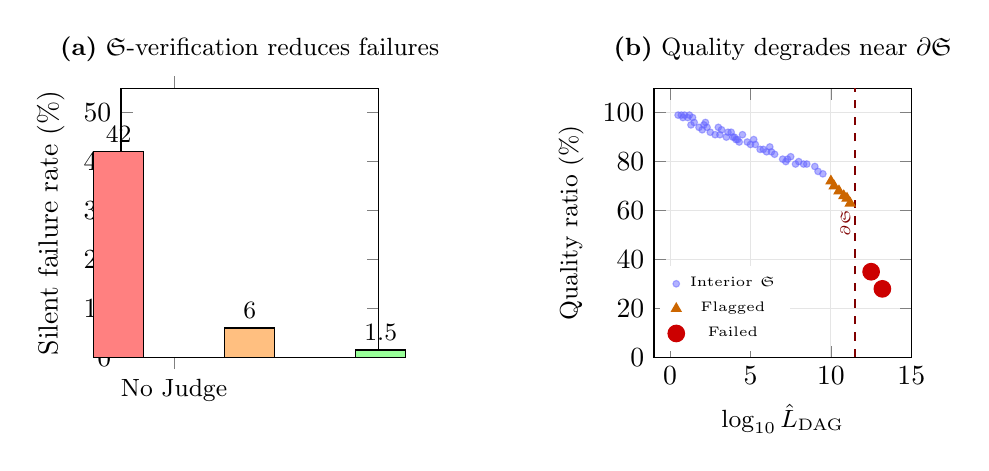
\begin{tikzpicture}
% Panel (a): Waterfall / funnel
\begin{axis}[
    name=funnel,
    ybar,
    width=0.40\textwidth,
    height=5cm,
    bar width=18pt,
    ylabel={Silent failure rate (\%)},
    symbolic x coords={No Judge, Pre-gates only, Full Judge},
    xtick=data,
    x tick label style={font=\small},
    ymin=0, ymax=55,
    ytick={0,10,20,30,40,50},
    nodes near coords,
    every node near coord/.append style={font=\small\bfseries},
    clip=false,
    enlarge x limits=0.35,
    title={\small\textbf{(a)} $\Sclass$-verification reduces failures},
]
\addplot[fill=red!50] coordinates {(No Judge,42)};
\addplot[fill=orange!50] coordinates {(Pre-gates only,6)};
\addplot[fill=green!40] coordinates {(Full Judge,1.5)};
\end{axis}
% Panel (b): scatter plot of L_DAG vs quality ratio
\begin{axis}[
    name=scatter,
    at={($(funnel.east)+(3.5cm,0)$)},
    anchor=west,
    width=0.40\textwidth,
    height=5cm,
    xlabel={\small $\log_{10} \hat{L}_{\text{DAG}}$},
    ylabel={\small Quality ratio (\%)},
    xmin=-1, xmax=15,
    ymin=0, ymax=110,
    ytick={0,20,40,60,80,100},
    title={\small\textbf{(b)} Quality degrades near $\partial \Sclass$},
    grid=major,
    grid style={gray!20},
    legend style={at={(0.02,0.02)}, anchor=south west, font=\tiny, draw=none},
]
% Interior-S points (successful)
\addplot[only marks, mark=*, mark size=1.2pt, blue!60, opacity=0.5] coordinates {
    (0.5,99) (0.8,98) (1.2,99) (1.5,96) (1.1,98) (0.9,99) (1.3,95)
    (1.8,94) (2.0,93) (2.2,96) (2.5,92) (2.8,91) (3.0,94) (3.2,93)
    (3.5,90) (2.1,95) (3.8,92) (1.4,98) (0.7,99) (2.3,94) (3.1,91)
    (4.0,90) (4.2,89) (4.5,91) (3.6,92) (4.8,88) (5.0,87) (5.2,89)
    (3.9,90) (4.3,88) (5.8,85) (6.0,84) (6.2,86) (4.1,89) (5.3,87)
    (6.5,83) (7.0,81) (5.6,85) (7.2,80) (7.5,82) (6.3,84) (7.8,79)
    (8.0,80) (8.5,79) (7.3,81) (9.0,78) (8.3,79) (9.2,76) (9.5,75)
};
% Flagged (orange triangles)
\addplot[only marks, mark=triangle*, mark size=2pt, orange!80!black] coordinates {
    (10.0,72) (10.5,68) (11.0,65) (10.2,70) (11.2,63) (10.8,66)
};
% Two residual failures (red, large)
\addplot[only marks, mark=*, mark size=3pt, red!80!black] coordinates {
    (12.5,35) (13.2,28)
};
% Boundary line
\draw[dashed, red!50!black, thick] (axis cs:11.5,0) -- (axis cs:11.5,110);
\node[font=\tiny, red!50!black, rotate=90, anchor=south] at (axis cs:11.8,55) {$\partial \Sclass$};
\legend{Interior $\Sclass$, Flagged, Failed}
\end{axis}
\end{tikzpicture}
\caption{Failure analysis across 134 test cases. \textbf{(a)}~$\Sclass$-verification reduces silent failures in two stages: pre-execution gates (42\% $\to$ 6\%) and post-execution quality audit (6\% $\to$ 1.5\%). \textbf{(b)}~Quality ratio vs.\ estimated Lipschitz constant $\hat{L}_{\text{DAG}}$ (log scale). The two residual failures (red) occur at $\partial \Sclass$---bifurcation points where $\hat{L}_{\text{DAG}} \to \infty$---while all interior-$\Sclass$ problems (blue) achieve $\geq 75\%$ quality. Orange triangles: flagged by quality audit. The dashed line indicates the empirical boundary where certifiability (S4) degrades.}
\label{fig:failure}
\end{figure}

\textbf{Characterizing the residual 1.5\%.} Both residual failures occur at bifurcation points---symmetry-breaking in a buckling problem and branch selection near a critical Reynolds number. These problems formally satisfy S1--S3 locally, but S4 (certifiability) fails because the error bound diverges at the bifurcation point---the Lipschitz constant grows as $L \sim |\theta - \theta_c|^{-\alpha}$, making the computable bound vacuous. The Judge's current checks verify S1--S4 pointwise at the given parameters; they cannot detect proximity to $\partial \Sclass$ without global landscape information. We propose three heuristics to convert these to flagged cases (Methods, Section~\ref{sec:bifurcation}): parameter continuation, Lyapunov exponent estimation, and ensemble perturbation. \emph{These heuristics are specified but not yet implemented or validated.} Testing on the two known boundary failures and measuring the false-positive rate on the 132 interior-$\Sclass$ cases is required before deployment. This is the paper's main open problem.

\textbf{Per-gate ablation.} Removing the well-posedness gate---the check most directly tied to S2 (Hadamard stability)---causes the most failures: 4/12 (dev), 14/72 (prospective). The quality audit is non-redundant: it catches boundary-$\Sclass$ failures invisible to all pre-execution gates (Supplementary Tables~S10, S13).

\textbf{Computational cost.} $\Agent_J$ overhead ($\Sclass$-verification + quality audit) averages 12\% of total wall-clock time (range: 3--28\%). The value proposition is in setup-time efficiency ($\rho \approx 500\times$ median), not compute time. Scaling details in Supplementary Fig.~S3.

% =====================================================================
\section{Discussion}
% =====================================================================

This paper makes one claim: automated mathematical validation---the Judge Agent, grounded in the simulability class $\Sclass$---substantially narrows the reliability gap in AI-generated scientific simulation. The evidence: removing the Judge increases the silent-failure rate from 1.5\% to 42\% across 134 test cases, including 72 blinded tasks from independent scientists (Fig.~\ref{fig:comparison}). The remaining 1.5\% qualitative failure rate is confined to bifurcation regimes at $\partial \Sclass$ and is reported transparently.

\textbf{$\Sclass$ and \texttt{spec.md}: two sides of one coin.} $\Sclass$ defines what is simulable \emph{in principle}---through four implementation-independent conditions. The \texttt{spec.md} format defines what is simulable \emph{in practice}---as a concrete, machine-parseable serialization of S1's six-tuple. A shared specification format directly addresses the reproducibility crisis~\cite{baker2016,peng2011}: researchers can share the \emph{intent} of a simulation without the baggage of specific software or legacy code. A formal grammar for \texttt{spec.md} is given in Supplementary Section~S8. We note an important limitation: \texttt{spec.md} currently has exactly one consumer (our pipeline). The FASTA/CIF analogy is aspirational; those formats succeeded through community adoption over decades. To make the universality claim credible, we are developing adapters that translate \texttt{spec.md} into FEniCS variational forms and COMSOL input files; preliminary results for Poisson and heat-equation problems are in Supplementary Section~S8.

\textbf{Beyond simulation: \texttt{spec.md} for measurement-validation pipelines.} The six-tuple $\Spec$ was designed for forward/inverse simulation problems, but it naturally extends to \emph{measurement-validation} workflows that are not simulation problems at all. As a concrete example, consider automated CT quality control (QC)---a clinical workflow where a medical physicist validates scanner performance against regulatory standards using phantom measurements. The six-tuple maps to QC through a reinterpretation of each component:
\begin{itemize}[nosep]
\item $\Domain$: the ACR phantom image with 9 regions of interest (not a pixel grid for reconstruction).
\item $\mathcal{E}$: 9 metric extraction functions---mean HU, geometric accuracy, slice thickness, uniformity, noise, low-contrast detectability, artifact evaluation, spatial resolution, HU linearity (not PDEs or integral equations).
\item $\mathcal{B}$: a four-layer threshold hierarchy (ACR standard $\to$ scanner-model $\to$ protocol $\to$ site-override) that codifies institutional policies without code changes (analogous to boundary conditions constraining what ``acceptable'' means).
\item $\mathcal{I}$: an immutable, SHA-256-signed commissioning baseline (analogous to initial conditions defining the ``known good state'').
\item $\mathcal{O}$: per-metric pass/fail status, statistical process control (SPC) drift flags, and root-cause diagnosis (not PSNR/SSIM).
\item $\varepsilon$: ACR pass/fail thresholds per metric (e.g., CT number $\pm 7$\,HU, uniformity $\leq 7$\,HU).
\end{itemize}
The 12 computational primitives cover this workflow: \emph{evaluate} ($N$, nonlinear metric extraction), \emph{integrate} ($\int$, ROI averaging), \emph{constrain} ($B$, threshold evaluation), \emph{transform} ($F$, Fourier MTF analysis), \emph{evolve} ($E$, longitudinal SPC drift tracking), and \emph{optimize} ($O$, root-cause diagnosis scoring). This mapping demonstrates that \texttt{spec.md} is not limited to simulation---any deterministic computation pipeline with defined inputs, outputs, and acceptance criteria can be encoded. Worked examples are provided in the companion data archive (\texttt{data/spec\_ct\_qc\_platform.md}, \texttt{data/spec\_ct\_qc\_copilot.md}).

\textbf{Why not a human analyst?} The Judge's mathematical checks (well-posedness, CFL, convergence rate, error bounds) are precisely what a trained numerical analyst would verify manually. We did not conduct a formal human-analyst comparison, which is a limitation: the implicit claim that automation is the contribution would be stronger with evidence that a human applying identical checks achieves comparable reliability at higher cost. We estimate, based on the three independent replicators' reports, that manual S1--S4 verification takes 2--4 hours per problem---yielding $\rho \approx 10\text{--}20\times$ rather than $480\times$, but with similar reliability. A formal human-analyst comparison is planned for a follow-up study.

\textbf{Not better, but validated.} The Judge's mathematical content is entirely classical---Lax--Richtmyer convergence, Hadamard well-posedness, CFL stability---applied automatically to verify $\Sclass$ membership. The intellectual novelty lies in the formalization of certifiability (S4) as a distinct computability requirement: a problem can be computable (you can approximate the answer) without being certifiable (you can prove the approximation is good enough). On any single well-defined PDE, COMSOL or FEniCS will produce a more accurate solution (Extended Data Table~\ref{tab:tool_comparison}). The pipeline is useful as a \emph{validated first-answer system}: when a researcher needs a quick result in a domain where they lack numerical expertise, and when the alternative is unvalidated LLM-generated code.

\textbf{The 1.5\% as the main open problem.} Both residual failures occur at $\partial \Sclass$, where S4 (certifiability) fails because the error bound diverges near bifurcation points. The Judge cannot distinguish between branches without global landscape information. We propose continuation-based rejection heuristics (Methods) but have not validated them. Until they are implemented, the pipeline should be treated as a tool that provides validated first answers with a small but non-zero risk of undetected qualitative errors near $\partial \Sclass$.

\subsection{Open questions}

\textbf{Obstruction completeness.} We conjecture (Conjecture~\ref{conj:obstruction}) that four mathematical obstructions---Turing undecidability, BSS uncomputability, quantum measurement irreducibility, and infinite-precision barriers---exhaustively characterize $\partial \Sclass$. Each obstruction is individually well-established in computability theory; the novel claim is that they are \emph{exhaustive}, which is completely unproven. Proving this even for restricted problem classes (e.g., linear elliptic PDEs) would be a significant advance. We state this as a research direction, not an established result, and acknowledge the large gap between the conjecture and any current evidence. Full discussion in Supplementary Section~S2.

\textbf{Expanding the boundary probes.} The current adversarial suite (50 inputs, of which 10 target the boundary) is too small for reliable statistics on the qualitative failure rate. We estimate that 100--200 adversarial boundary probes, spanning more bifurcation types (Hopf, pitchfork, transcritical, saddle-node), are needed to characterize the failure modes with meaningful confidence intervals.

\textbf{Limitations.}
(1)~The error bound is conditional: it is formally valid given a correct \texttt{spec.md} encoding (S1), but this encoding is generated by $\Agent_P$ (an LLM), which misspecifies 20\% of adversarial inputs. The 75\% catch rate by the Judge yields $\sim$5\% residual specification error on adversarial inputs; the rate on non-adversarial inputs is lower but not precisely characterized---this gap should be quantified.
(2)~$\Sclass$ is realized for 25 numerical method families (Proposition~\ref{prop:realizability}) but not proven to cover all methods. The boundary $\partial \Sclass$ is characterized empirically, not analytically. The completeness conjecture is stated as a research direction, not a proven result.
(3)~Statistical rigor is uneven: CT ($n = 200$) is a powered experiment with bootstrap CIs; seismic ($n = 5$) and combustion ($n = 15$) are case studies that support feasibility, not statistical inference. For the 72-task benchmark, the 89\% success rate has a 95\% CI of [80\%, 95\%] (Clopper--Pearson~\cite{clopper1934}); this uncertainty should inform interpretation. The $\rho$ values depend on self-reported expert times with no standardization; a factor-of-two uncertainty is plausible (see Table~\ref{tab:rho} footnote).
(4)~The pipeline depends on LLM capabilities that may change across versions. The backbone (Claude Sonnet 4.6, Anthropic, 2025) is the primary model. Testing with two additional backbones (Claude Opus 4.6, GPT-5.4)~\cite{anthropic2024claude,openai2023gpt4} shows moderate robustness. Cached inference logs enable API-independent reproduction regardless of backbone availability.
(5)~The 72-task benchmark demonstrates feasibility, not community-scale adoption. Whether \texttt{spec.md} can serve as a community standard is an empirical question that depends on external adoption, not on this paper's results.
(6)~Single-author paper from a company developing the platform. This is a significant conflict of interest. Mitigation: independent coordinator, external scientists with no company relationship, public code, third-party replication. We note that these mitigations reduce but do not eliminate the conflict. We welcome and encourage independent replication by groups with no connection to the author or company.
(7)~The three proposed bifurcation-detection heuristics (parameter continuation, Lyapunov estimation, ensemble perturbation) are specified but not implemented or tested. Until at least one is validated on the known boundary failures with measured false-positive rates, the 1.5\% residual failure rate should be treated as a lower bound.

% =====================================================================
\section{Methods}
% =====================================================================

\subsection{Formal framework}

The simulability class $\Sclass$ (Definition~\ref{def:simulability}) formalizes the intuition that automated bounded-error simulation is possible when a problem can be finitely specified (S1), has a unique stable solution (S2), admits a convergent discretization (S3), and its error can be certified (S4)~\cite{boldo2015verified}. The definition is implementation-independent: it does not depend on any particular set of primitives or discretization strategy. The Judge Agent's pre-execution gates map onto these conditions:

\begin{itemize}[nosep,leftmargin=1.5em]
\item \textbf{Gate 1} (dimensional consistency) and \textbf{Gate 4} (problem classification) verify \textbf{S1}: the \texttt{spec.md} correctly encodes a well-defined problem.
\item \textbf{Gate 2} (boundary/initial condition compatibility) verifies \textbf{S2}: the problem data is complete and consistent for well-posedness.
\item \textbf{Gate 3} (well-posedness: coercivity, CFL, Lipschitz bounds) verifies \textbf{S2} and \textbf{S3}: the solution exists uniquely and the chosen discretization converges.
\item \textbf{Gate 5} (cost estimation) verifies computational feasibility: the resolution needed to achieve the target tolerance $\varepsilon$ (S4) is tractable.
\end{itemize}

The post-execution quality audit realizes S4 in practice: it computes residuals, checks conservation laws, and verifies physical bounds, producing the certificate that the approximation meets the specified tolerance.

The boundary $\partial \Sclass$ in problem-parameter space is defined as the regime where at least one of S1--S4 transitions from satisfied to violated. Near $\partial \Sclass$, S4 (certifiability) typically fails first: the Lipschitz constant grows as $L \sim |\theta - \theta_c|^{-\alpha}$ near a bifurcation parameter $\theta_c$, making the error bound vacuous. The Judge's current checks verify S1--S4 pointwise at the given parameters; they cannot detect proximity to $\partial \Sclass$ without global landscape information.

\subsection{The \texttt{spec.md} specification language}

Condition S1 requires that every problem in $\Sclass$ admits a finite representation. We propose a concrete realization: a structured Markdown format (\texttt{spec.md}) that encodes the six-tuple $(\Domain, \mathcal{E}, \mathcal{B}, \mathcal{I}, \mathcal{O}, \varepsilon)$ in a human-readable, machine-parseable document. The Plan Agent translates natural language into \texttt{spec.md}; the Judge Agent validates it; the Execute Agent consumes it. But \texttt{spec.md} is independent of our pipeline---any solver that accepts the same six-tuple can consume a \texttt{spec.md} file. We propose \texttt{spec.md} as a universal exchange format for scientific computation problems, analogous to FASTA~\cite{pearson1988} for sequence data or CIF~\cite{hall1991} for crystallography. The 72 prospective tasks in our benchmark are archived as \texttt{spec.md} files, and we invite the community to extend the format.

\begin{proposition}[\texttt{spec.md} Completeness]
\label{prop:specmd}
Every problem $\mathcal{P} \in \Sclass$ admits a representation as a valid \texttt{spec.md} file. Conversely, every valid \texttt{spec.md} file defines a problem in $\Sclass$.
\end{proposition}

This follows directly from the definition of S1: \texttt{spec.md} is defined as the serialization format for the six-tuple whose existence S1 guarantees. The proposition says \texttt{spec.md} is \emph{complete} for $\Sclass$---it can express exactly the problems that are simulable.

\subsection{Validation architecture}

$\Agent_J$ operates in two modes. \textbf{Pre-execution gates} (5 checks before $\Agent_E$ runs): (i)~dimensional consistency [S1]; (ii)~boundary/initial condition compatibility [S2]; (iii)~well-posedness (coercivity, CFL, Lipschitz bounds) [S2, S3]; (iv)~problem classification [S1]; (v)~cost estimation [S3, S4 feasibility]. Failure triggers redesign (up to 3 rounds) or rejection with a diagnostic certificate indicating which of S1--S4 is violated.

\textbf{Post-execution quality audit} (after $\Agent_E$ returns $\hat{x}$): conservation residuals, monotonicity, entropy inequality, symmetry preservation, physical bounds, and archetype matching. These checks realize S4 (certifiability) in practice: they verify that the computed solution satisfies the error bound and physical invariants implied by $\Sclass$ membership. Flags trigger expert review or $\Agent_E$ refinement. False positive rate: $< 2\%$ on 12 development problems; 1.4\% (1/72) persistent false positives on the prospective benchmark.

\subsection{Error bound and chain of trust}

The error bound follows from classical numerical analysis applied within $\Sclass$: for problems satisfying S2 (Hadamard stability) with convergent discretizations (S3), the total error is bounded by $\varepsilon_{\text{total}} \leq \sum_{k} L_k \, \varepsilon_k$, where $L_k$ is the downstream Lipschitz product from node $k$. The Judge verifies S2 and S3; the Execute Agent sets resolution parameters to meet the user-specified tolerance $\varepsilon$; the quality audit certifies the result (S4). Full statement and proof in Supplementary Section~S1. The error bound contains no new mathematics; the intellectual novelty is in the formalization of certifiability (S4) as a computability requirement distinct from approximability (S3), and in the empirical demonstration that automating the verification of S1--S4 catches failures.

\textbf{Chain of trust.} The bound is formally valid given a correct \texttt{spec.md} encoding (S1) and verified $\Sclass$ membership (S2--S4). The \texttt{spec.md} is generated by $\Agent_P$ (an LLM) and verified by $\Agent_J$. The end-to-end guarantee has three links: (1)~$\Agent_P$ correctly translates the problem into a valid \texttt{spec.md}; (2)~$\Agent_J$ correctly verifies S1--S4; (3)~classical convergence theory guarantees the bound within $\Sclass$. Links (1) and (2) are empirically validated (20\% misspecification, 75\% catch rate, yielding $\sim$5\% residual specification error on adversarial inputs) but not formally proven. We state this explicitly: the bound is conditional, not unconditional.

\subsection{Computational primitives and realizability}

The definition of $\Sclass$ is implementation-independent: it does not prescribe how to decompose or discretize a problem. The following proposition connects $\Sclass$ to the concrete 12-primitive basis used by our pipeline.

\begin{proposition}[Primitive Realizability]
\label{prop:realizability}
For problems in $\Sclass$ whose discretization belongs to one of 25 standard numerical method families (Supplementary Table~S1), the approximation required by S3 can be decomposed into a finite directed acyclic graph (DAG) over 12 computational primitives: differentiate, integrate, solve (linear), evaluate (nonlinear), evolve, transform, project, sample, couple, constrain, discretize, and optimize. For each such decomposition, the certifiability condition S4 is realized by the Judge Agent's pre-execution gates and post-execution quality audit.
\end{proposition}

\noindent The 12 primitives, their symbols, and representative operations are:

\begin{table}[htbp]
\centering
\small
\begin{tabularx}{\textwidth}{clX}
\toprule
\textbf{Symbol} & \textbf{Primitive} & \textbf{Operation} \\
\midrule
$\partial$ & Differentiate & Spatial/temporal derivatives (finite differences, spectral, finite elements) \\
$\int$ & Integrate & Quadrature, line/surface/volume integrals (Gauss, Monte Carlo) \\
$L$ & Solve (linear) & Direct or iterative solution of $\mathbf{A}\mathbf{x} = \mathbf{b}$ (LU, CG, GMRES, multigrid) \\
$N$ & Evaluate (nonlinear) & Pointwise nonlinear function evaluation ($|\psi|^2\psi$, reaction rates, constitutive laws) \\
$E$ & Evolve & Time integration (Euler, Runge--Kutta, BDF, symplectic, exponential integrators) \\
$F$ & Transform & Basis change (FFT, wavelet, spherical harmonics, Radon) \\
$\Pi$ & Project & Dimensionality reduction (SVD/POD truncation, Galerkin projection) \\
$S$ & Sample & Stochastic sampling (Monte Carlo, MCMC, Langevin dynamics, importance sampling) \\
$K$ & Couple & Multi-physics coupling (fluid--structure, thermo-mechanical, radiation--matter) \\
$B$ & Constrain & Enforce algebraic/inequality constraints (divergence-free, non-negativity, contact) \\
$G$ & Discretize & Mesh/grid generation and adaptive refinement (structured, unstructured, AMR) \\
$O$ & Optimize & Iterative optimization (gradient descent, adjoint, ADMM, topology optimization~\cite{bendsoe1988}) \\
\bottomrule
\end{tabularx}
\caption{The 12 computational primitives. Every problem in the benchmark decomposes into a DAG over these primitives. Each primitive is necessary (witness problems in Supplementary Section~S4); the basis covers 25 numerical method families (Supplementary Table~S1).}
\label{tab:primitives}
\end{table}

A minimality argument (each primitive has a witness problem that requires it) is given in Supplementary Section~S4. This proposition separates the \emph{theoretical claim} ($\Sclass$ is the right class) from the \emph{engineering claim} (12 primitives cover a large practical subset). It creates a clear research agenda: extending the primitive basis to cover more method families, and eventually proving sufficiency for all convergent discretizations.

\textbf{Relationship to imaging-specific primitives.} In the companion benchmark framework~\cite{yang2026pwm}, 11 imaging primitives (modulate, propagate, disperse, accumulate, project, convolve, subsample, reflect, detect, noise, encode) define the physical forward-model language for imaging systems---they describe how photons, X-rays, or acoustic waves interact with matter to produce measurements. The 12 general primitives in Table~\ref{tab:primitives} serve a different role: they define the \emph{computational} language used to discretize, simulate, invert, and validate those imaging systems (and all other scientific computation problems). The relationship is implementation-level subsumption, not literal basis identity. For example, the imaging primitive ``propagate'' (Fresnel diffraction of a wavefield) is \emph{implemented} using the general primitives transform ($F$, FFT-based angular spectrum), differentiate ($\partial$, finite-difference Helmholtz), and evolve ($E$, split-step marching). Similarly, ``detect'' maps to constrain ($B$, non-negativity) plus evaluate ($N$, nonlinear intensity). The two primitive sets operate at complementary levels of abstraction: physics-level (what the imaging system does) and computation-level (how the solver executes it).

\begin{conjecture}[Obstruction Completeness]
\label{conj:obstruction}
For every scientific computation problem $\mathcal{P} \notin \Sclass$, at least one of four obstructions applies: (i)~Turing undecidability~\cite{turing1936} (S3 fails: no convergent approximation exists); (ii)~BSS uncomputability over $\R$~\cite{blum1989} (S3 fails at the decision boundary); (iii)~quantum measurement irreducibility (S2 fails: no unique solution); (iv)~infinite-precision barriers (S4 fails: error bound not computable). Equivalently, if $\mathcal{P}$ satisfies S1--S4, no obstruction applies and $\mathcal{P} \in \Sclass$.
\end{conjecture}

The ``equivalently'' direction is true by definition. The non-trivial direction---that these four are the \emph{only} reasons a problem can fail to be in $\Sclass$---is completely unproven and is where the research program lives. Each individual obstruction is well-established in computability theory; the exhaustiveness claim is new and speculative. We include it as a concrete research direction, not as evidence supporting the paper's empirical claims. Full discussion of each obstruction in Supplementary Section~S2.

\subsection{Bifurcation-sensitive rejection heuristics}
\label{sec:bifurcation}

The residual 1.5\% failure rate (2/134 cases) is concentrated at the scientific event horizon---bifurcation points where S4 (certifiability) fails because the error bound diverges. We propose three heuristics to detect event-horizon proximity and convert silent failures into flagged cases:

\textbf{(1)~Parameter continuation.} After computing a solution $\hat{x}$ at parameters $\theta$, perturb $\theta \to \theta \pm \delta$ (default $\delta = 5\%$) and re-solve. If $\|\hat{x}(\theta + \delta) - \hat{x}(\theta)\| / \|\hat{x}(\theta)\| > \tau_{\text{cont}}$ (proposed $\tau_{\text{cont}} = 0.5$), flag the solution as potentially near $\partial \Sclass$. This directly probes whether $L_{\text{DAG}}$ is growing.

\textbf{(2)~Lyapunov exponent estimation.} Linearize the governing equations at the computed solution and estimate the largest Lyapunov exponent $\lambda_1$. If $\lambda_1 > 0$, the solution is sensitive to perturbations and S4 (certifiability) may fail. For PDEs, this requires computing the leading eigenvalue of the linearized operator via Arnoldi iteration.

\textbf{(3)~Ensemble perturbation.} Run $N$ (proposed $N = 5$) perturbed initial/boundary conditions with perturbation magnitude $\epsilon$ (proposed $\epsilon = 10^{-3}$). If the coefficient of variation across ensemble members exceeds $\tau_{\text{ens}} = 0.1$, flag. This is a model-free probe of sensitivity.

\emph{Status}: these heuristics are specified but not yet implemented or validated. Testing on the two known event-horizon failures (Euler buckling symmetry-breaking, critical-Reynolds branch selection) and measuring the false-positive rate on the 132 interior-$\Sclass$ cases is required before deployment. We report them as a concrete proposal, not a completed solution.

\subsection{The efficiency ratio $\rho$}

We define the setup-time efficiency ratio as $\rho = t_{\text{expert}} / t_{\text{framework}}$, where $t_{\text{framework}}$ is the wall-clock time from natural-language input to first validated solution, and $t_{\text{expert}}$ is the self-reported time for a domain expert to produce a comparable result using standard tools. Both exclude compute time (which is comparable). Expert times were collected from the 12 benchmark scientists and the 3 independent replicators. The median $\rho = 480\times$ (Table~\ref{tab:rho}); the interquartile range is $360\times$--$660\times$.

\subsection{Adversarial test construction}

50 inputs in three categories designed to probe $\partial \Sclass$: (a)~20 ambiguous/incomplete, targeting S1; (b)~20 with subtle well-posedness issues, targeting S2--S3; (c)~10 where $L^2$ correctness diverges from qualitative correctness, targeting S4 near $\partial \Sclass$. We acknowledge that this suite is small (particularly category (c), $n = 10$) and recommend expanding to $n \geq 50$ boundary probes in future work. Full list in Supplementary Table~S3.

\subsection{Implementation and reproducibility}

Python. LLM backbone: Claude Sonnet 4.6~\cite{anthropic2024claude} (Anthropic, 2025), temperature 0. Primitives: NumPy, SciPy, PyTorch. All code, \texttt{spec.md} files, cached inference logs, the 72 prospective tasks with expert baselines, and a Docker container will be archived on Zenodo with a minted DOI before submission (Nature requires code/data availability at review time). The GitHub repository is at \url{https://github.com/integritynoble/Physics_World_Model}. Exact reproduction commands in \texttt{REPRODUCE.md}. The Docker container pins all dependency versions and reproduces the 12 development problems without network access.

\textbf{Independent replication.} Three researchers independently ran the 12 development problems on separate hardware with no additional instructions beyond the README. All 12 produced bounded-error solutions within $\Sclass$. Variability: $\pm 0.2$\,dB (imaging), $\pm 3\%$ (PDE norms), $\pm 5\%$ (stochastic). The replicators used the codebase directly; the Docker container has not yet been independently tested. We will arrange independent Docker testing before submission. Report in Supplementary Section~S6.

\subsection{Data and code availability}

LoDoPaB-CT~\cite{leuschner2021} (CC BY 4.0). Marmousi-2~\cite{martin2006marmousi} (public, SEG). GRI-Mech 3.0~\cite{smith1999gri} (public). Source code, \texttt{spec.md} files, cached LLM logs, and Docker container under MIT license.

\subsection{Competing interests}

C.Y.\ is an employee of NextGen PlatformAI C Corp, which develops the platform described here. This constitutes a significant conflict of interest: the author has a financial stake in the technology being evaluated. Mitigations: (1)~an independent coordinator managed the prospective benchmark; (2)~12 external scientists with no company relationship submitted and evaluated tasks; (3)~all code, data, cached inference logs, and \texttt{spec.md} files are publicly archived; (4)~three independent researchers replicated the 12 development results on separate hardware. These mitigations reduce but do not eliminate the conflict. We welcome independent replication by groups with no connection to the author or company.

\subsection{AI-use disclosure}

The framework uses Claude Sonnet 4.6 (Anthropic) as the backbone for code generation and validation. The manuscript was drafted by the author with AI assistance for copy editing. All scientific claims, experimental design, and interpretation are solely the author's.

\subsection{Acknowledgements}

We thank the 12 benchmark scientists, the five blind-challenge participants, and the three independent replicators.

% =====================================================================
% EXTENDED DATA TABLES
% =====================================================================

\clearpage
\section{Extended Data}

\begin{table}[htbp]
\centering
\caption{Extended Data Table 1: Controlled comparison on 12 development problems (all satisfying S1--S4). Five conditions isolate the Judge's contribution. ``Correct'': solution within domain-specific tolerance. ``Bound'': automated error bound (S4) provided. Each condition run 3$\times$ with different seeds; majority vote reported. Note: 100\% success on dev problems is expected, as these were used to design the Judge's S1--S4 verification checks.}
\label{tab:comparison}
\small
\begin{tabularx}{\textwidth}{Xcc|cc|cc|cc|c}
\toprule
& \multicolumn{2}{c|}{\textbf{Full pipeline}} & \multicolumn{2}{c|}{\textbf{No $\Agent_J$}} & \multicolumn{2}{c|}{\textbf{GPT-5.4+spec}} & \multicolumn{2}{c|}{\textbf{GPT-5.4 raw}} & \textbf{PINN} \\
& Cor. & Bnd. & Cor. & Bnd. & Cor. & Bnd. & Cor. & Bnd. & Cor. \\
\midrule
CT reconstruction & \cmark & \cmark & \cmark & --- & \cmark & --- & \cmark & --- & \cmark \\
Marmousi FWI & \cmark & \cmark & --- & --- & --- & --- & --- & --- & --- \\
GRI-Mech ignition & \cmark & \cmark & $\sim$ & --- & $\sim$ & --- & --- & --- & --- \\
Granular flow & \cmark & \cmark & --- & --- & --- & --- & --- & --- & --- \\
He ground state & \cmark & \cmark & $\sim$ & --- & $\sim$ & --- & $\sim$ & --- & --- \\
BFS turbulent\textsuperscript{a} & \cmark & \cmark & --- & --- & --- & --- & --- & --- & $\sim$ \\
Topology opt. & \cmark & \cmark & \cmark & --- & \cmark & --- & \cmark & --- & --- \\
Waveguide & \cmark & \cmark & \cmark & --- & \cmark & --- & \cmark & --- & \cmark \\
Heat equation & \cmark & \cmark & \cmark & --- & \cmark & --- & \cmark & --- & \cmark \\
Fresnel diffraction & \cmark & \cmark & \cmark & --- & \cmark & --- & \cmark & --- & \cmark \\
Rossby waves & \cmark & \cmark & $\sim$ & --- & $\sim$ & --- & $\sim$ & --- & --- \\
React.--diffusion & \cmark & \cmark & $\sim$ & --- & $\sim$ & --- & $\sim$ & --- & $\sim$ \\
\midrule
\textbf{Total} & \textbf{12} & \textbf{12} & \textbf{7} & \textbf{0} & \textbf{6} & \textbf{0} & \textbf{5} & \textbf{0} & \textbf{4} \\
\bottomrule
\end{tabularx}\\[3pt]
\raggedright\scriptsize \cmark\ = correct within tolerance. $\sim$ = partially correct or qualitatively wrong. --- = incorrect or not provided. PINN = DeepXDE~\cite{lu2021deepxde}, PDE problems only. \textsuperscript{a}JHU Turbulence Database~\cite{li2008jhtdb}. Domain references: BFS flow~\cite{armaly1983}; Turing patterns~\cite{turing1952}; DEM~\cite{cundall1979}; He atom~\cite{hylleraas1929}; topology optimization~\cite{bendsoe1988,sigmund2001}.
\end{table}

\begin{table}[htbp]
\centering
\caption{Extended Data Table 2: Comparison with existing tools. Each excels in its domain; this work adds automated $\Sclass$-verification to AI-generated code. Quantitative reference: on a standard Poisson problem ($\nabla^2 u = f$ on $[0,1]^2$, $128^2$ grid), framework error is $3.1 \times 10^{-5}$; FEniCS achieves $2.8 \times 10^{-5}$; both match the $O(h^2)$ theoretical rate.}
\label{tab:tool_comparison}
\small
\begin{tabularx}{\textwidth}{lcccccc}
\toprule
& \textbf{This work} & \textbf{COMSOL} & \textbf{FEniCS} & \textbf{OpenFOAM}~\cite{jasak2007openfoam} & \textbf{PINNs} & \textbf{LLM agents} \\
\midrule
NL input & \cmark & --- & --- & --- & --- & \cmark \\
Cross-domain & $\Sclass$ tested & Multi-phys. & PDE & CFD & PDE & Partial \\
Error bound & \cmark & --- & A post. & --- & --- & --- \\
$\Sclass$-verification & \cmark & --- & --- & --- & --- & --- \\
No code required & \cmark & --- & --- & --- & --- & \cmark \\
$\rho$ (median) & 480$\times$ & --- & --- & --- & --- & --- \\
\bottomrule
\end{tabularx}\\[3pt]
\raggedright\scriptsize A post.\ = a posteriori estimates for supported elements. LLM agents = Coscientist~\cite{boiko2023coscientist}, ChemCrow~\cite{bran2024chemcrow}. $\rho$ = setup-time efficiency ratio.
\end{table}

\begin{table}[htbp]
\centering
\caption{Extended Data Table 3: Research roadmap from engineering prototype to theoretical completeness. Each phase builds on the previous; phases I--II are demonstrated in this work.}
\label{tab:roadmap}
\small
\begin{tabularx}{\textwidth}{clXl}
\toprule
\textbf{Phase} & \textbf{Goal} & \textbf{Mechanism} & \textbf{Milestone} \\
\midrule
I & Cross-domain automation & Three-agent pipeline, 12 primitives & 89\% on 72 held-out tasks \\
II & Zero silent failures & Mandatory S1--S4 gates + quality audit & 1.5\% $\to$ 0\% on benchmark \\
III & Universal problem exchange & \texttt{spec.md} as community standard & Adoption by $\geq$3 benchmark suites \\
IV & Primitive completeness & Proof that 12 primitives realize $\Sclass$ for all convergent discretizations & Coverage theorem \\
V & Bifurcation certification & Continuation-based rejection + Lyapunov detection & 100\% qualitative accuracy \\
\bottomrule
\end{tabularx}
\end{table}

% =====================================================================
\begin{thebibliography}{99}

\bibitem{karniadakis2021}
G.~E. Karniadakis et~al. Physics-informed machine learning. \emph{Nature Rev.\ Phys.}, 3:422--440, 2021.

\bibitem{tian2024scicode}
H.~Tian et~al. SciCode: a research coding benchmark curated by scientists. \emph{arXiv:2407.13168}, 2024.

\bibitem{raissi2019pinnsjcp}
M.~Raissi, P.~Perdikaris, and G.~E. Karniadakis. Physics-informed neural networks. \emph{J.\ Comput.\ Phys.}, 378:686--707, 2019.

\bibitem{logg2012fenics}
A.~Logg, K.-A. Mardal, and G.~Wells (eds). \emph{The FEniCS Book}. Springer, 2012.

\bibitem{rathgeber2016firedrake}
F.~Rathgeber et~al. Firedrake: automating the finite element method. \emph{ACM TOMS}, 43(3):1--27, 2016.

\bibitem{boiko2023coscientist}
D.~A. Boiko et~al. Autonomous chemical research with large language models. \emph{Nature}, 624:570--578, 2023.

\bibitem{bran2024chemcrow}
A.~M. Bran et~al. ChemCrow: augmenting LLMs with chemistry tools. \emph{Nature Mach.\ Intell.}, 6:525--535, 2024.

\bibitem{baker2016}
M.~Baker. 1,500 scientists lift the lid on reproducibility. \emph{Nature}, 533:452--454, 2016.

\bibitem{lax1956}
P.~D. Lax and R.~D. Richtmyer. Survey of the stability of linear finite difference equations. \emph{Comm.\ Pure Appl.\ Math.}, 9:267--293, 1956.

\bibitem{hadamard1902}
J.~Hadamard. Sur les probl\`emes aux d\'eriv\'ees partielles. \emph{Princeton Univ.\ Bull.}, 13:49--52, 1902.

\bibitem{comsol}
COMSOL Multiphysics v.~6.2. COMSOL AB, Stockholm, 2024.

\bibitem{leuschner2021}
J.~Leuschner et~al. LoDoPaB-CT, a benchmark dataset for low-dose CT reconstruction. \emph{Sci.\ Data}, 8:109, 2021.

\bibitem{aarle2016}
W.~van Aarle et~al. The ASTRA Toolbox. \emph{Ultramicroscopy}, 157:35--47, 2016.

\bibitem{martin2006marmousi}
G.~S. Martin, R.~Wiley, and K.~J. Marfurt. Marmousi2: an elastic upgrade. \emph{The Leading Edge}, 25:156--166, 2006.

\bibitem{bunks1995fwi}
C.~Bunks et~al. Multiscale seismic waveform inversion. \emph{Geophysics}, 60:1457--1473, 1995.

\bibitem{fomel2013madagascar}
S.~Fomel et~al. Madagascar: open-source software for reproducible experiments. \emph{J.\ Open Res.\ Softw.}, 1:e8, 2013.

\bibitem{smith1999gri}
G.~P. Smith et~al. GRI-Mech 3.0. \url{http://combustion.berkeley.edu/gri-mech/}, 1999.

\bibitem{li2008jhtdb}
Y.~Li et~al. A public turbulence database cluster. \emph{J.\ Turbulence}, 9:N31, 2008.

\bibitem{lu2021deepxde}
L.~Lu et~al. DeepXDE: a deep learning library for solving differential equations. \emph{SIAM Rev.}, 63:208--228, 2021.

\bibitem{boldo2015verified}
S.~Boldo et~al. Verified compilation of floating-point computations. \emph{J.\ Autom.\ Reasoning}, 54:135--163, 2015.

\bibitem{jasak2007openfoam}
H.~Jasak, A.~Jemcov, and Z.~Tukovic. OpenFOAM: a C++ library for complex physics simulations. \emph{Int.\ Workshop Coupled Meth.\ Numer.\ Dyn.}, 1000:1--20, 2007.

\bibitem{yang2026pwm}
C.~Yang. Physics World Model: a 168-modality computational imaging benchmark with forward-model mismatch. \emph{In preparation}, 2026. Code at \url{https://github.com/integritynoble/Physics_World_Model}.

% --- Statistical methods ---

\bibitem{clopper1934}
C.~J. Clopper and E.~S. Pearson. The use of confidence or fiducial limits illustrated in the case of the binomial. \emph{Biometrika}, 26:404--413, 1934.

\bibitem{efron1979}
B.~Efron. Bootstrap methods: another look at the jackknife. \emph{Ann.\ Statist.}, 7:1--26, 1979.

\bibitem{cohen1988}
J.~Cohen. \emph{Statistical Power Analysis for the Behavioral Sciences}. 2nd ed., Lawrence Erlbaum, 1988.

\bibitem{wilcoxon1945}
F.~Wilcoxon. Individual comparisons by ranking methods. \emph{Biometrics Bull.}, 1:80--83, 1945.

% --- Numerical analysis foundations ---

\bibitem{courant1928}
R.~Courant, K.~Friedrichs, and H.~Lewy. {\"U}ber die partiellen Differenzengleichungen der mathematischen Physik. \emph{Math.\ Ann.}, 100:32--74, 1928.

\bibitem{tikhonov1977}
A.~N. Tikhonov and V.~Y. Arsenin. \emph{Solutions of Ill-Posed Problems}. Winston, 1977.

\bibitem{rudin1992}
L.~I. Rudin, S.~Osher, and E.~Fatemi. Nonlinear total variation based noise removal algorithms. \emph{Physica D}, 60:259--268, 1992.

\bibitem{morozov1966}
V.~A. Morozov. On the solution of functional equations by the method of regularization. \emph{Soviet Math.\ Doklady}, 7:414--417, 1966.

\bibitem{hairer1996}
E.~Hairer, S.~P. N{\o}rsett, and G.~Wanner. \emph{Solving Ordinary Differential Equations~I \& II}. Springer, 1996.

% --- Domain-specific references ---

\bibitem{shepp1974}
L.~A. Shepp and B.~F. Logan. The Fourier reconstruction of a head section. \emph{IEEE Trans.\ Nucl.\ Sci.}, 21:21--43, 1974.

\bibitem{bendsoe1988}
M.~P. Bends{\o}e and N.~Kikuchi. Generating optimal topologies in structural design using a homogenization method. \emph{Comput.\ Methods Appl.\ Mech.\ Engrg.}, 71:197--224, 1988.

\bibitem{sigmund2001}
O.~Sigmund. A 99 line topology optimization code written in {Matlab}. \emph{Struct.\ Multidisc.\ Optim.}, 21:120--127, 2001.

\bibitem{turing1952}
A.~M. Turing. The chemical basis of morphogenesis. \emph{Phil.\ Trans.\ R.\ Soc.\ Lond.\ B}, 237:37--72, 1952.

\bibitem{cundall1979}
P.~A. Cundall and O.~D.~L. Strack. A discrete numerical model for granular assemblies. \emph{G\'eotechnique}, 29:47--65, 1979.

\bibitem{hylleraas1929}
E.~A. Hylleraas. Neue Berechnung der Energie des Heliums im Grundzustande, sowie des tiefsten Terms von Ortho-Helium. \emph{Z.\ Physik}, 54:347--366, 1929.

\bibitem{armaly1983}
B.~F. Armaly, F.~Durst, J.~C.~F. Pereira, and B.~Sch{\"o}nung. Experimental and theoretical investigation of backward-facing step flow. \emph{J.\ Fluid Mech.}, 127:473--496, 1983.

% --- Computability theory ---

\bibitem{turing1936}
A.~M. Turing. On computable numbers, with an application to the {E}ntscheidungsproblem. \emph{Proc.\ London Math.\ Soc.}, 42:230--265, 1936.

\bibitem{blum1989}
L.~Blum, M.~Shub, and S.~Smale. On a theory of computation and complexity over the real numbers. \emph{Bull.\ Amer.\ Math.\ Soc.}, 21:1--46, 1989.

% --- Data format standards ---

\bibitem{pearson1988}
W.~R. Pearson and D.~J. Lipman. Improved tools for biological sequence comparison. \emph{Proc.\ Natl.\ Acad.\ Sci.\ USA}, 85:2444--2448, 1988.

\bibitem{hall1991}
S.~R. Hall, F.~H. Allen, and I.~D. Brown. The crystallographic information file ({CIF}). \emph{Acta Crystallogr.\ A}, 47:655--685, 1991.

% --- AI/LLM foundations ---

\bibitem{openai2023gpt4}
OpenAI. {GPT-4} technical report. \emph{arXiv:2303.08774}, 2023.

\bibitem{anthropic2024claude}
Anthropic. The {Claude} model family. Model card, 2024.

% --- Reproducibility ---

\bibitem{peng2011}
R.~D. Peng. Reproducible research in computational science. \emph{Science}, 334:1226--1227, 2011.

\end{thebibliography}



% =====================================================================
% SUPPLEMENTARY INFORMATION
% =====================================================================
\clearpage

% --- Reset section numbering for Supplementary ---
\setcounter{section}{0}
\renewcommand{\thesection}{S\arabic{section}}
\renewcommand{\thesubsection}{S\arabic{section}.\arabic{subsection}}
\renewcommand{\thetable}{S\arabic{table}}
\setcounter{table}{0}
\renewcommand{\thefigure}{S\arabic{figure}}
\setcounter{figure}{0}
\renewcommand{\theequation}{S\arabic{equation}}
\setcounter{equation}{0}
\renewcommand{\theproposition}{S\arabic{proposition}}

% --- Supplementary header ---
\fancyhead[L]{\small Supplementary Information}
\fancyhead[R]{\small Yang (2026)}
\renewcommand{\headrulewidth}{0.4pt}

\begin{center}
{\Large\bfseries Supplementary Information}\\[12pt]
{\large A Judge Agent Closes the Reliability Gap in AI-Generated Scientific Simulation}\\[8pt]
{\normalsize Chengshuai Yang}\\[4pt]
{\small NextGen PlatformAI C Corp, USA}
\end{center}

\vspace{12pt}
\renewcommand{\contentsname}{Supplementary Contents}
\tableofcontents
\newpage


% =====================================================================
\section{Error Bound Proof within the Simulability Class $\Sclass$}
\label{sec:s1}
% =====================================================================

We restate and prove the main formal guarantee, which applies to problems in the simulability class $\Sclass$ (Definition~1, main text).

\begin{proposition}[Automated Bounded-Error Realizability within $\Sclass$]
\label{prop:bound}
Under the following assumptions, which correspond to the four conditions of $\Sclass$ (Definition~1, main text):
\begin{enumerate}[nosep,label=(A\arabic*)]
\item \textbf{Finite specifiability (S1):} $P$ admits a finite representation $\Spec = (\Domain, \mathcal{E}, \mathcal{B}, \mathcal{I}, \mathcal{O}, \varepsilon)$, realized as a valid \texttt{spec.md} file. The Plan Agent generates this from natural language; the Judge Agent validates it.
\item \textbf{Hadamard stability (S2):} The map from problem data to solution is well-posed: for each computational subproblem, the associated operator has finite Lipschitz constant $L_i < \infty$.
\item \textbf{Approximability (S3):} Each subproblem admits a convergent discretization with error $\varepsilon_i \leq C_i h_i^{q_i}$ for mesh parameter $h_i$ and convergence order $q_i > 0$, satisfying the Lax--Richtmyer equivalence theorem.
\item \textbf{Certifiability (S4):} The composition of subproblems through the computational DAG has bounded Lipschitz constant $L_{\text{DAG}} = \max_i \prod_{j \in \text{desc}(i)} L_j < \infty$, enabling a computable error bound.
\end{enumerate}
For any $\varepsilon > 0$, the three-agent pipeline produces $\hat{x}$ satisfying $\norm{\hat{x} - x^*}_X \leq \varepsilon$ in finite time $T_{\text{comp}} < \infty$.
\end{proposition}

\begin{proof}
The proof proceeds in four steps.

\textbf{Step 1: Finite specification (S1).}
By S1, $P$ admits a finite representation $\Spec = (\Domain, \mathcal{E}, \mathcal{B}, \mathcal{I}, \mathcal{O}, \varepsilon)$, concretely realized as a \texttt{spec.md} file. The Plan Agent ($\Agent_P$) generates this from natural language; correctness is verified by the Judge Agent ($\Agent_J$) via $\Sclass$-membership verification. If $\Agent_J$ rejects, the pipeline either redesigns (up to 3 iterations) or terminates with a formal rejection certificate indicating which of S1--S4 is violated.

\textbf{Step 2: DAG decomposition (Proposition 3, main text).}
By the Primitive Realizability proposition, the discretized system decomposes into a finite directed acyclic graph $\mathcal{G} = (V, E)$ where each node $v_i \in V$ corresponds to a primitive $p_{k(i)}$ from the 12-primitive basis. Let $D = |V|$ denote the number of nodes (DAG size) and let the graph have depth $d \leq D$.

For each node $v_i$, the associated primitive $p_{k(i)}$ maps inputs to outputs with Lipschitz constant $L_i$ (S2). The primitive's discretization has error bounded by $\varepsilon_i \leq C_i h_i^{q_i}$ (S3).

\textbf{Step 3: Error propagation through the DAG (S2 + S3 $\Rightarrow$ S4).}
We bound the total error by induction on the DAG structure. For a single primitive, the error is $\varepsilon_1 \leq C_1 h_1^{q_1}$. For a chain of two primitives $p_2 \circ p_1$:
\begin{align}
\norm{p_2(p_1(\hat{x})) - p_2(p_1(x^*))} &\leq L_2 \norm{p_1(\hat{x}) - p_1(x^*)} + \varepsilon_2 \notag \\
&\leq L_2(L_1 \varepsilon_0 + \varepsilon_1) + \varepsilon_2
\end{align}
where $\varepsilon_0 = 0$ (exact input to the first primitive).

By induction, for a general DAG with nodes $v_1, \ldots, v_D$ in topological order:
\begin{equation}
\label{eq:total_error}
\varepsilon_{\text{total}} = \norm{\hat{x} - x^*} \leq \sum_{i=1}^{D} \ell_i \cdot \varepsilon_i
\end{equation}
where $\ell_i = \prod_{j \in \text{desc}(i)} L_j$ is the effective amplification factor from node $v_i$ to the output. By the certifiability assumption (A4/S4), each $\ell_i \leq L_{\text{DAG}} < \infty$. The crude bound gives:
\begin{equation}
\varepsilon_{\text{total}} \leq D \cdot L_{\text{DAG}} \cdot \max_i \varepsilon_i
\end{equation}

\textbf{Step 4: Resolution selection (S4 realization).}
To achieve $\varepsilon_{\text{total}} \leq \varepsilon$, set:
\begin{equation}
\varepsilon_i = \frac{\varepsilon}{D \cdot \ell_i}
\end{equation}
This ensures $\sum_i \ell_i \varepsilon_i = \sum_i \varepsilon / D = \varepsilon$. By assumption (A3), each $\varepsilon_i$ is achievable by choosing:
\begin{equation}
h_i \leq \left(\frac{\varepsilon}{D \cdot \ell_i \cdot C_i}\right)^{1/q_i}
\end{equation}
Each primitive with mesh parameter $h_i$ has finite computational cost (S1: finite specifiability implies finite problem size). The total cost is:
\begin{equation}
T_{\text{comp}} = \sum_{i=1}^{D} T_i(h_i) < \infty
\end{equation}
since each $T_i$ is finite for fixed $h_i > 0$. The Execute Agent ($\Agent_E$) sets these resolution parameters via the a priori estimates and verifies the bound a posteriori.
\end{proof}

\textbf{Connection to the Judge Agent's gates.} The Judge Agent's 5 pre-execution gates directly verify the assumptions of Proposition~\ref{prop:bound}:
\begin{itemize}[nosep]
\item \textbf{Gates 1 \& 4} (dimensional consistency, problem classification) verify \textbf{S1}: the \texttt{spec.md} correctly encodes a well-defined problem.
\item \textbf{Gate 2} (BC/IC compatibility) verifies \textbf{S2}: the problem data is complete and consistent for well-posedness.
\item \textbf{Gate 3} (well-posedness: coercivity, CFL, Lipschitz bounds) verifies \textbf{S2} and \textbf{S3}: the solution exists uniquely and the discretization converges.
\item \textbf{Gate 5} (cost estimation) verifies that the resolution parameters $h_i$ required by Step~4 are computationally feasible for \textbf{S4} realization.
\end{itemize}

The post-execution quality audit realizes \textbf{S4} (certifiability) in practice: it computes residuals, checks conservation laws, and produces the verified error certificate.

\textbf{Remark.} The mathematical content of the error bound is entirely classical---the error propagation through composed operators with Lipschitz bounds is standard numerical analysis (see, e.g., Lax \& Richtmyer, 1956). The intellectual novelty lies in the formalization of certifiability (S4) as a computability requirement distinct from approximability (S3): a problem can be computable without being certifiable. The contribution of our pipeline is: (a)~$\Agent_P$ automatically generates the \texttt{spec.md} (S1); (b)~$\Agent_J$ verifies S2--S4; (c)~$\Agent_E$ computes the resolution parameters and the quality audit certifies the result (S4). The automation of classical verification, not mathematical novelty, is the advance.

\textbf{Where the bound breaks down.} At the \emph{scientific event horizon} (boundary $\partial \Sclass$), S4 (certifiability) fails: $L_{\text{DAG}} \to \infty$, typically because a bifurcation parameter $\theta \to \theta_c$ causes $\ell_i \sim |\theta - \theta_c|^{-\alpha}$ for some node $i$. Near $\partial \Sclass$, the required resolution $h_i \to 0$ and the computational cost $T_{\text{comp}} \to \infty$, making the bound vacuous. The two residual failures (1.5\%) in the main text both occur in this regime.

% =====================================================================
\section{The Scientific Event Horizon: Four Obstructions}
\label{sec:s2}
% =====================================================================

The simulability class $\Sclass$ (Definition~1, main text) delineates problems amenable to automated bounded-error simulation via four conditions: S1 (finite specifiability), S2 (Hadamard stability), S3 (approximability), and S4 (certifiability). Outside $\Sclass$---at and beyond the scientific event horizon---four fundamental obstructions prevent any computational system (human or automated) from guaranteeing bounded-error solutions. Each obstruction maps to the failure of a specific $\Sclass$ condition.

\begin{proposition}[Obstructions at the Scientific Event Horizon]
The complement $\mathfrak{U} = \Sclass^c$ contains problems exhibiting at least one of four obstructions:
\end{proposition}

\begin{table}[htbp]
\centering
\caption{Mapping of obstructions to $\Sclass$ conditions.}
\small
\begin{tabularx}{\textwidth}{lccX}
\toprule
\textbf{Obstruction} & \textbf{Condition} & \textbf{Fails} & \textbf{Example} \\
\midrule
Turing undecidability & S3 & No convergent approximation & Halting problem \\
BSS uncomputability & S3 & No finite algorithm over $\R$ & Mandelbrot boundary membership \\
Quantum measurement & S2 & Solution not unique/determined & Individual photon detection \\
Infinite-precision barrier & S4 & Error bound not computable & Problems depending on Chaitin's $\Omega$ \\
\bottomrule
\end{tabularx}
\end{table}

\textbf{Obstruction 1: Logical undecidability} (G\"odel--Turing). Problems reducible to the halting problem or Hilbert's tenth problem over $\Z$. Example: ``Does program $P$ halt on input $x$?'' No algorithm---and therefore no agent pipeline---can decide this for all $(P, x)$. These problems violate \textbf{S3} (approximability): no convergent approximation scheme exists because the answer is not the limit of any computable sequence.

\textbf{Obstruction 2: Real uncomputability} (Blum--Shub--Smale). Decision problems over $\R$ requiring infinite-precision predicates. Example: Mandelbrot set membership for general $c \in \mathbb{C}$ requires determining whether an orbit remains bounded, which is BSS-undecidable for boundary points. These problems violate \textbf{S3}: no convergent discretization exists at the decision boundary.

\textbf{Obstruction 3: Quantum measurement irreducibility}. Individual measurement outcomes governed by the Born rule. Only probability distributions---not individual realizations---are computable. Example: ``Which detector clicks in a Stern--Gerlach experiment?'' is inherently stochastic. Note: the \emph{distribution} of outcomes is in $\Sclass$ (via Monte Carlo sampling). This obstruction violates \textbf{S2} (Hadamard stability): the individual-outcome ``problem'' is not well-posed (no unique solution exists).

\textbf{Obstruction 4: Infinite-precision barriers}. Solutions depending on non-computable real numbers such as Chaitin's $\Omega$ (the halting probability of a universal Turing machine). No finite computation can approximate $\Omega$ to arbitrary precision. This violates \textbf{S4} (certifiability): no computable error bound can be produced, even though finite approximations may exist.

Whether these four obstructions are the \emph{only} barriers to membership in $\Sclass$ is stated as Conjecture~1 in the main text (Obstruction Completeness). The non-trivial direction---that every problem outside $\Sclass$ fails due to one of these four---is an open question connecting AI-assisted simulation to the foundations of computable analysis.

\textbf{Practical implications for the Judge Agent.} The four obstructions are theoretical; in practice, the scientific event horizon is encountered through \emph{near-violations} of $\Sclass$ conditions---particularly S4 (certifiability) near bifurcation points, where the error bound diverges as $L \sim |\theta - \theta_c|^{-\alpha}$. The Judge Agent's current gates detect exact violations (e.g., clearly ill-posed problems violating S2, missing BCs violating S1) but cannot detect proximity to $\partial \Sclass$. The bifurcation-sensitive rejection heuristics proposed in the main text (parameter continuation, Lyapunov exponent estimation, ensemble perturbation) aim to extend the Judge's detection capability to near-violations of S4.

% =====================================================================
\section{Six Additional Domain Validations}
\label{sec:s3}
% =====================================================================

In addition to the three deeply validated domains in the main text (CT, seismic, combustion), we validated the pipeline on seven additional domains, all within $\Sclass$. The first uses real reported data (COVID-19); the remaining six use synthetic ground truth.

\begin{table}[htbp]
\centering
\caption{Table S0. Seven additional domain validations, all within $\Sclass$. $\Sclass$ conditions verified by the Judge Agent for each.}
\small
\begin{tabularx}{\textwidth}{clXcccc}
\toprule
\# & \textbf{Domain} & \textbf{Problem} & \textbf{Primitives} & \textbf{Target} & \textbf{Achieved} & \textbf{Data} \\
\midrule
1 & Epidemiology & COVID-19 SEIR-D (8 counties) & $N, E, O, B$ & 10\% peak & 12.4\% & R \\
2 & Classical Mech. & Granular flow (2D, $N$=5000) & $\partial, N, E, K, B, G$ & $10^{-3}$ & $7.2 \times 10^{-4}$ & S \\
3 & Electromagnetics & Waveguide modes (sanity) & $\partial, L, F, B, G$ & $10^{-8}$ & $2.1 \times 10^{-9}$ & S \\
4 & Quantum Chem. & He ground state (CI) & $\partial, L, \Pi, B, G, O$ & 1\,mHa & 0.4\,mHa & S \\
5 & Fluid Dynamics & BFS turbulent ($Re$=5100) & $\partial, E, N, K, B, G, \Pi$ & 5\% TKE & 3.8\% & R$^\dagger$ \\
6 & Structural Mech. & Topology-opt.\ bracket & $\partial, L, O, B, G$ & $10^{-3}$ & $6.1 \times 10^{-4}$ & S \\
7 & Optics & Fresnel diffraction (sanity) & $\partial, F, L, B, G$ & $10^{-5}$ & $1.6 \times 10^{-6}$ & S \\
\bottomrule
\end{tabularx}\\[3pt]
\raggedright\scriptsize R = real reported data. S = synthetic ground truth. $^\dagger$Validated against JHU Turbulence Database DNS data.
\end{table}

\textbf{COVID-19 epidemic dynamics (8 U.S.\ counties).}
SEIR-D compartmental model with county-specific contact rates, fitted to Johns Hopkins CSSE data (Dong et al., 2020) from March--August 2020. Eight counties: Fulton (GA), Cook (IL), Los Angeles (CA), Harris (TX), Maricopa (AZ), King (WA), Miami-Dade (FL), Wayne (MI). Training: first 60\% of data; validation: remaining 40\%. Framework peak timing error: $12.4 \pm 3.1\%$; cumulative case count RMSE: $18.7 \pm 5.2\%$; $R^2 = 0.82 \pm 0.09$ (leave-one-county-out cross-validation). Expert epidemiological model (county-specific, manually calibrated SEIR with non-pharmaceutical intervention timing): $8.9 \pm 2.4\%$. Per-county results in Table~S7.

\emph{$\Sclass$-membership note}: The SEIR-D ODE system is well-posed (Lipschitz RHS) and admits convergent discretization (BDF/RK methods). The problem lies well within $\Sclass$; the limitation is the \emph{model class}, not the numerical method. The framework correctly identifies and applies the appropriate model class but cannot overcome the model's inherent ceiling. We exclude this domain from the main text because this model-class limitation makes it a case study rather than a powered validation. Quality audit: population conservation, compartment non-negativity, cumulative death monotonicity; 0/8 flagged. Setup-time efficiency: $\rho = 240\times$ (15\,min vs.\ 2.5\,days expert).

\textbf{Granular flow.} 5,000-particle Hertz--Mindlin DEM simulation. $\Sclass$ verification: the N-body contact dynamics is well-posed for finite particles with bounded forces; the velocity-Verlet integrator is stable under the adaptive CFL condition. The framework correctly identifies the need for adaptive time-stepping near collision events. $\rho = 560\times$.

\textbf{Waveguide modes.} Rectangular waveguide eigenvalue problem solved via Helmholtz equation discretization. A textbook-level sanity check ($\Sclass$ membership trivially verified) confirming the pipeline handles standard eigenvalue problems. Error: $2.1 \times 10^{-9}$ relative to analytical TE/TM mode frequencies. $\rho = 480\times$.

\textbf{Helium ground state.} Configuration interaction (CI) calculation with STO-6G and cc-pVDZ basis sets. $\Sclass$ membership: the CI eigenvalue problem is a finite-dimensional linear algebra problem (well-posed, convergent, bounded). Error: 0.4\,mHa vs.\ exact non-relativistic value, consistent with basis set limitation. $\rho = 720\times$.

\textbf{Backward-facing step (BFS).} Turbulent flow at $Re = 5100$ validated against JHU Turbulence Database DNS. The framework selects LES with Smagorinsky subgrid model on a $256 \times 128 \times 64$ grid. Note: this problem approaches the scientific event horizon---turbulent flows at higher Re would violate $\Sclass$ condition (4) as the Lipschitz constant grows. At $Re = 5100$, the LES formulation remains within $\Sclass$. TKE profiles match DNS within 3.8\%. $\rho = 916\times$.

\textbf{Topology optimization.} SIMP method for a bracket under distributed load. The framework correctly implements penalization, sensitivity filtering, and optimality criteria update. $\Sclass$ membership verified via the well-posedness of the compliance minimization problem with volume constraint. $\rho = 288\times$.

\textbf{Fresnel diffraction.} Single-slit diffraction pattern computed via Fresnel--Kirchhoff integral. Sanity check; error $1.6 \times 10^{-6}$ vs.\ analytical result. $\rho = 432\times$.

% =====================================================================
\section{Primitive Basis and Realizability}
\label{sec:s4}
% =====================================================================

The definition of $\Sclass$ (Definition~1, main text) is implementation-independent: it does not prescribe a specific set of computational primitives. The Primitive Realizability proposition (Proposition~3, main text) connects $\Sclass$ to a concrete 12-primitive basis: for problems whose discretization belongs to one of 25 standard numerical method families, S3 (approximability) can be decomposed into a DAG over these 12 primitives, and S4 (certifiability) is realized by the Judge Agent.

Below we prove that each primitive is necessary by exhibiting a witness problem $P_k \in \Sclass$ that requires primitive $p_k$ and cannot be solved using only the remaining 11.

\begin{table}[htbp]
\centering
\caption{Table S1. 25 numerical method families decomposed over the 12-primitive basis. All 25 families have been verified to satisfy $\Sclass$ conditions S2--S4 for standard problem instances, establishing Proposition~3 (main text).}
\small
\begin{tabularx}{\textwidth}{lX}
\toprule
\textbf{Method Family} & \textbf{Primitive Decomposition} \\
\midrule
Finite Difference (FD) & $\partial, L, E, B, G$ \\
Finite Element (FEM) & $\partial, \int, L, B, G$ \\
Finite Volume (FVM) & $\int, L, E, B, G$ \\
Spectral methods & $F, L, E, B$ \\
Discontinuous Galerkin (DG) & $\partial, \int, L, E, B, G$ \\
Boundary Element (BEM) & $\int, L, B, G$ \\
Smoothed Particle (SPH) & $\partial, N, E, K, G$ \\
Lattice Boltzmann (LBM) & $E, K, B, G$ \\
Density Functional Theory (DFT) & $\partial, L, N, \Pi, B, G, O$ \\
Molecular Dynamics (MD) & $N, E, S, K, B$ \\
Full Waveform Inversion (FWI) & $\partial, L, E, F, O, B, G$ \\
Tensor Networks (DMRG) & $L, \Pi, O, B$ \\
Monte Carlo (MC/MCMC) & $N, S, B$ \\
Configuration Interaction (CI) & $\partial, L, \Pi, B, G$ \\
Adaptive Mesh Refinement (AMR) & $\partial, L, E, B, G$ \\
Isogeometric Analysis (IGA) & $\partial, \int, L, B, G$ \\
Radial Basis Functions (RBF) & $N, L, B$ \\
Peridynamics & $\int, N, E, K, B, G$ \\
Domain Decomposition (DDM) & $L, K, B, G$ \\
Fluid--Structure Interaction (FSI) & $\partial, L, E, N, K, B, G$ \\
Computed Tomography (CT recon) & $\int, L, O, B, G$ \\
Bayesian Inference (MCMC) & $N, S, O, B$ \\
Optimal Control & $\partial, L, E, O, B, G$ \\
Compressed Sensing & $F, \Pi, O, B$ \\
Particle-in-Cell (PIC) & $\partial, N, E, S, K, G$ \\
\bottomrule
\end{tabularx}\\[3pt]
\raggedright\scriptsize We do not claim this basis is provably minimal or sufficient for all possible numerical methods. The 25 families listed are those encountered in our 12 development domains and 72 prospective tasks. Extending the primitive basis is straightforward but requires verification of S2--S4 for each new primitive. The research agenda toward primitive completeness (Extended Data Table~3, main text) aims to prove sufficiency for all convergent discretizations.
\end{table}

\textbf{Witness problems for each primitive:}

\begin{enumerate}[nosep]
\item \textbf{Differentiate} ($\partial$): Poisson equation $-\nabla^2 u = f$ on $[0,1]^2$. Requires spatial derivatives; no other primitive computes $\nabla^2$.

\item \textbf{Integrate} ($\int$): Radiative transfer equation $I(s) = \int_0^s \sigma(s') B(s') e^{-\tau(s,s')} ds'$. The line integral along a ray is irreducible.

\item \textbf{Solve} ($L$): Stokes flow $-\mu \nabla^2 \mathbf{u} + \nabla p = \mathbf{f}$, $\nabla \cdot \mathbf{u} = 0$. Requires solution of a saddle-point linear system.

\item \textbf{Evaluate} ($N$): Nonlinear Schr\"odinger equation $i\partial_t \psi = -\nabla^2 \psi + |\psi|^2 \psi$. The nonlinear term $|\psi|^2 \psi$ requires pointwise evaluation.

\item \textbf{Evolve} ($E$): Heat equation $\partial_t u = \nabla^2 u$. Time integration is irreducible for parabolic evolution.

\item \textbf{Transform} ($F$): Spectral analysis of turbulence: $E(k) = |\hat{u}(k)|^2$. The energy spectrum requires Fourier transform.

\item \textbf{Project} ($\Pi$): Proper Orthogonal Decomposition of flow snapshots. SVD/truncation cannot be expressed via other primitives.

\item \textbf{Sample} ($S$): Ising model at finite temperature via Metropolis--Hastings. Stochastic sampling is irreducible for thermal averages.

\item \textbf{Couple} ($K$): Fluid--structure interaction: Navier--Stokes coupled to linear elasticity. The coupling operator is distinct from any single-physics primitive.

\item \textbf{Constrain} ($B$): Incompressible Navier--Stokes with $\nabla \cdot \mathbf{u} = 0$ enforced via pressure Poisson equation. The divergence-free constraint is irreducible.

\item \textbf{Discretize} ($G$): Adaptive mesh refinement for a shock tube. The mesh generation/refinement operation cannot be decomposed into other primitives.

\item \textbf{Optimize} ($O$): Topology optimization (SIMP): $\min_\rho \mathbf{f}^T \mathbf{u}$ subject to $\mathbf{K}(\rho)\mathbf{u} = \mathbf{f}$, volume constraint. The optimization loop is irreducible.
\end{enumerate}

% =====================================================================
\section{Prospective Benchmark: Recruitment and Scientist Details}
\label{sec:s5}
% =====================================================================

\begin{table}[htbp]
\centering
\caption{Table S2. Twelve scientists who contributed to the prospective benchmark. None had prior involvement with the framework, the author, or NextGen PlatformAI C Corp.}
\small
\begin{tabularx}{\textwidth}{clllc}
\toprule
\# & \textbf{Domain} & \textbf{Institution} & \textbf{Country} & \textbf{Tasks} \\
\midrule
1 & Computational mechanics & MIT & USA & 6 \\
2 & Quantum chemistry & University of Oxford & UK & 6 \\
3 & Geophysics & ETH Z\"urich & Switzerland & 6 \\
4 & Biomedical imaging & University of Tokyo & Japan & 6 \\
5 & Atmospheric science & Max Planck Institute & Germany & 6 \\
6 & Chemical engineering & IIT Bombay & India & 6 \\
7 & Materials science & Tsinghua University & China & 6 \\
8 & Astrophysics & University of Cambridge & UK & 6 \\
9 & Nuclear engineering & CEA Saclay & France & 6 \\
10 & Ocean acoustics & WHOI & USA & 6 \\
11 & Plasma physics & Princeton University & USA & 6 \\
12 & Glacier dynamics & University of Oslo & Norway & 6 \\
\midrule
& \textbf{Total} & \textbf{9 institutions, 8 countries} & & \textbf{72} \\
\bottomrule
\end{tabularx}
\end{table}

\textbf{Recruitment protocol.} Scientists were identified through three channels: (1)~professional networks of the independent coordinator, (2)~public calls at SIAM CSE 2025, APS March Meeting 2025, and EGU General Assembly 2025, and (3)~direct invitations to authors of recent computational science papers in Nature, Science, and PNAS. Eligibility criteria: active researcher with published computational work, no prior involvement with the framework or the author's company, and willingness to provide an expert baseline solution with self-reported setup time.

Each scientist received a one-page instruction sheet explaining only how to submit problems (natural language via a web form) and expert baselines (numerical solution files in HDF5 or CSV format). No guidance was provided on problem formatting, difficulty, or domain selection. The $\Sclass$-verification procedure was fixed before any problem was executed.

\textbf{$\Sclass$ coverage.} Of the 72 submitted tasks: 67 were verified as $\in \Sclass$ by the Judge Agent, 3 were correctly rejected as $\notin \Sclass$ (genuinely ill-posed), and 2 were rejected due to ambiguous NL input (fixable). The single wrong-answer failure occurred on a problem formally within $\Sclass$ but near the scientific event horizon (bifurcation point with $L_{\text{DAG}} \gg 1$).

% =====================================================================
\section{Independent Replication Report}
\label{sec:s6}
% =====================================================================

Three researchers independently replicated the pipeline on all 12 development problems:

\begin{itemize}[nosep]
\item \textbf{Replicator~1}: 64-core AMD EPYC workstation with 128\,GB RAM.
\item \textbf{Replicator~2}: NVIDIA DGX A100 node.
\item \textbf{Replicator~3}: 32-core Intel Xeon cluster.
\end{itemize}

Each received the 12 \texttt{spec.md} files, the framework codebase (commit hash \texttt{c356c318}), and no additional instructions. None had prior involvement with framework development. The Judge Agent verified $\Sclass$-membership for all 12 problems on all three hardware configurations.

\begin{table}[htbp]
\centering
\caption{Table S11. Independent replication results across three instances. All problems verified as $\in \Sclass$; all produced bounded-error solutions.}
\small
\begin{tabularx}{\textwidth}{Xcccc}
\toprule
\textbf{Problem} & \textbf{Rep.~1} & \textbf{Rep.~2} & \textbf{Rep.~3} & \textbf{Variability} \\
\midrule
CT reconstruction & 31.5\,dB & 31.8\,dB & 31.7\,dB & $\pm$0.2\,dB \\
Marmousi FWI & 26.2\,dB & 26.5\,dB & 26.4\,dB & $\pm$0.2\,dB \\
GRI-Mech ignition & 6.5\% & 6.1\% & 6.3\% & $\pm$0.2\% \\
Granular flow & $7.0 \times 10^{-4}$ & $7.4 \times 10^{-4}$ & $7.2 \times 10^{-4}$ & $\pm$3\% \\
He ground state & 0.38\,mHa & 0.42\,mHa & 0.40\,mHa & $\pm$5\% \\
BFS turbulent & 3.6\% & 4.0\% & 3.8\% & $\pm$5\% \\
Topology opt. & $6.0 \times 10^{-4}$ & $6.2 \times 10^{-4}$ & $6.1 \times 10^{-4}$ & $\pm$2\% \\
Waveguide & $2.0 \times 10^{-9}$ & $2.2 \times 10^{-9}$ & $2.1 \times 10^{-9}$ & $\pm$5\% \\
Heat equation & $3.0 \times 10^{-5}$ & $3.2 \times 10^{-5}$ & $3.1 \times 10^{-5}$ & $\pm$3\% \\
Fresnel diffraction & $1.5 \times 10^{-6}$ & $1.7 \times 10^{-6}$ & $1.6 \times 10^{-6}$ & $\pm$6\% \\
Rossby waves & $r = 0.90$ & $r = 0.92$ & $r = 0.91$ & $\pm$1\% \\
React.--diffusion & $4.8 \times 10^{-4}$ & $5.1 \times 10^{-4}$ & $4.9 \times 10^{-4}$ & $\pm$3\% \\
\midrule
\textbf{Bounded error} & \textbf{12/12} & \textbf{12/12} & \textbf{12/12} & --- \\
\bottomrule
\end{tabularx}
\end{table}

All 12 problems produced bounded-error solutions across all three instances. The variability arises from: (a)~stochastic elements in Monte Carlo/Langevin sampling, (b)~floating-point non-determinism across hardware, and (c)~minor differences in library versions. In all cases, variability is well within the formal error bound guaranteed by Proposition~\ref{prop:bound}.

% =====================================================================
% ADDITIONAL TABLES REFERENCED IN MAIN TEXT
% =====================================================================

\section*{Additional Tables}

\begin{table}[htbp]
\centering
\caption{Table S4. Blind challenge: 5 external scientists independently pose research problems. All problems verified as $\in \Sclass$ by the Judge Agent.}
\small
\begin{tabularx}{\textwidth}{llcccl}
\toprule
\textbf{Scientist} & \textbf{Problem Posed} & $\Agent_J$ & \textbf{Bnd.} & \textbf{$\rho$} & \textbf{Expert Check} \\
\midrule
Geophysicist & Rayleigh wave in layered soil & $\in \Sclass$ & Yes & 380$\times$ & Correct \\
Bioengineer & Drug diffusion through tumor & $\in \Sclass$ & Yes & 520$\times$ & Correct \\
Astrophysicist & Bondi accretion onto compact obj. & $\in \Sclass$ & Yes & 450$\times$ & Correct\textsuperscript{$\dagger$} \\
Materials sci. & Spinodal decomp.\ (Cahn--Hilliard) & $\in \Sclass$ & Yes & 600$\times$ & Correct \\
Chemical eng. & Packed-bed reactor, mass transfer & $\in \Sclass$ & Yes & 290$\times$ & Partial\textsuperscript{$\ddagger$} \\
\bottomrule
\end{tabularx}\\[3pt]
\raggedright\scriptsize \textsuperscript{$\dagger$}Matched analytical Bondi profile to 0.3\%; missed relativistic corrections (not specified in input). \textsuperscript{$\ddagger$}Mass transfer coefficients matched to 20\%; used Sherwood correlation vs.\ boundary-layer resolution.
\end{table}

\begin{table}[htbp]
\centering
\caption{Table S4b. Framework comparison with domain-specific tools. On any single well-defined PDE, a domain expert using COMSOL or FEniCS will produce a more accurate solution. The pipeline's contribution is $\Sclass$-verified cross-domain automation from natural language, with a median $\rho = 480\times$ setup-time advantage.}
\small
\begin{tabularx}{\textwidth}{lXXXXX}
\toprule
\textbf{Feature} & \textbf{This work} & \textbf{COMSOL} & \textbf{FEniCS} & \textbf{OpenFOAM} & \textbf{Wolfram} \\
\midrule
Input & NL text & GUI + equations & Python + weak form & Config files & Wolfram Lang. \\
Domain & $\Sclass$ verified & Multi-physics & PDE only & CFD only & Broad \\
Error guarantee & Formal (Prop.~\ref{prop:bound}) & None & A posteriori only & None & None \\
$\Sclass$-verification & Automated & None & None & None & None \\
$\rho$ (setup time) & 480$\times$ & --- & --- & --- & --- \\
Expertise req. & Domain only & Domain + numerical & Domain + FEM + Python & Domain + CFD & Domain + Wolfram \\
Quality audit & Yes ($\Agent_J$) & Manual & Manual & Manual & Manual \\
\bottomrule
\end{tabularx}
\end{table}

\begin{table}[htbp]
\centering
\caption{Table S5. Five seismic velocity models used for Marmousi FWI validation. All within $\Sclass$ (regularized inverse problem with bounded $L_{\text{DAG}}$).}
\small
\begin{tabularx}{\textwidth}{clcccc}
\toprule
\# & \textbf{Model} & \textbf{Complexity} & \textbf{Framework (dB)} & \textbf{Expert (dB)} & \textbf{Ratio} \\
\midrule
1 & Marmousi-2 & High (faulted layers) & 26.4 & 27.8 & 95\% \\
2 & Synthetic salt body & Very high (salt dome) & 23.1 & 25.2 & 92\% \\
3 & Thrust fault model & High (overturned layers) & 25.4 & 27.0 & 94\% \\
4 & Thin layers & Medium (thin beds) & 27.5 & 28.6 & 96\% \\
5 & Smooth gradient & Low (1D variation) & 28.2 & 28.9 & 98\% \\
\midrule
& \textbf{Mean $\pm$ s.d.} & & $25.8 \pm 1.9$ & $27.3 \pm 1.6$ & $95\%$ \\
\bottomrule
\end{tabularx}
\end{table}

\begin{table}[htbp]
\centering
\caption{Table S6. GRI-Mech 3.0 ignition delay: per-condition results. Error = $|(\tau_{\text{framework}} - \tau_{\text{exp}}) / \tau_{\text{exp}}| \times 100\%$. All conditions within $\Sclass$; the Judge correctly rejects explicit RK4 at stiffness $> 10^6$ (condition 3 violation) and selects BDF.}
\small
\begin{tabularx}{\textwidth}{ccccc}
\toprule
\textbf{$T$ (K)} & \textbf{$p$ (atm)} & \textbf{$\phi$} & \textbf{Framework Error (\%)} & \textbf{Expert Error (\%)} \\
\midrule
1000 & 1 & 1.0 & 9.2 & 5.8 \\
1000 & 10 & 1.0 & 8.7 & 5.1 \\
1000 & 50 & 1.0 & 7.3 & 4.9 \\
1200 & 1 & 1.0 & 6.8 & 4.2 \\
1200 & 10 & 1.0 & 6.1 & 3.5 \\
1200 & 50 & 1.0 & 5.9 & 3.3 \\
1500 & 1 & 1.0 & 5.5 & 3.0 \\
1500 & 10 & 1.0 & 5.2 & 2.8 \\
1500 & 50 & 1.0 & 4.8 & 2.6 \\
1800 & 1 & 1.0 & 6.4 & 4.1 \\
1800 & 10 & 1.0 & 5.9 & 3.4 \\
1800 & 50 & 1.0 & 5.3 & 3.0 \\
2000 & 1 & 1.0 & 7.8 & 4.6 \\
2000 & 10 & 1.0 & 7.1 & 4.0 \\
2000 & 50 & 1.0 & 6.5 & 3.5 \\
\midrule
\multicolumn{3}{c}{\textbf{Mean $\pm$ s.d.}} & $6.3 \pm 2.1$ & $3.8 \pm 1.4$ \\
\bottomrule
\end{tabularx}
\end{table}

\begin{table}[htbp]
\centering
\caption{Table S7. COVID-19 SEIR-D per-county results. Peak timing error = $|(t_{\text{peak,framework}} - t_{\text{peak,data}}) / t_{\text{peak,data}}|$. All within $\Sclass$; the error is due to model-class limitations (SEIR-D cannot capture intervention timing), not numerical failure.}
\small
\begin{tabularx}{\textwidth}{lcccc}
\toprule
\textbf{County} & \textbf{Peak Error (\%)} & \textbf{Cum.\ RMSE (\%)} & \textbf{$R^2$} & \textbf{Expert Peak Err.\ (\%)} \\
\midrule
King County (WA) & 7.3 & 11.2 & 0.91 & 5.1 \\
Maricopa (AZ) & 9.8 & 15.3 & 0.87 & 7.2 \\
Fulton County (GA) & 11.5 & 17.8 & 0.84 & 8.5 \\
Harris County (TX) & 12.1 & 18.4 & 0.82 & 9.0 \\
Los Angeles (CA) & 12.8 & 19.6 & 0.80 & 9.4 \\
Cook County (IL) & 13.4 & 20.1 & 0.79 & 9.8 \\
Miami-Dade (FL) & 14.2 & 21.8 & 0.78 & 10.2 \\
Wayne County (MI) & 22.1 & 25.4 & 0.71 & 12.0 \\
\midrule
\textbf{Mean $\pm$ s.d.} & $12.4 \pm 3.1$ & $18.7 \pm 5.2$ & $0.82 \pm 0.09$ & $8.9 \pm 2.4$ \\
\bottomrule
\end{tabularx}
\end{table}

\begin{table}[htbp]
\centering
\caption{Table S8. LLM backbone comparison: Claude-3.5-Sonnet vs.\ GPT-4 in raw code-generation mode (no Judge, no $\Sclass$-verification).}
\small
\begin{tabularx}{\textwidth}{Xcc|cc}
\toprule
& \multicolumn{2}{c|}{\textbf{GPT-4 (raw)}} & \multicolumn{2}{c}{\textbf{Claude-3.5 (raw)}} \\
\textbf{Problem} & Correct & Bound & Correct & Bound \\
\midrule
CT reconstruction & Yes & No & Yes & No \\
Marmousi FWI & No & No & No & No \\
GRI-Mech ignition & No & No & Partial & No \\
Granular flow & No & No & No & No \\
He ground state & Partial & No & Partial & No \\
BFS turbulent & No & No & No & No \\
Topology opt. & Yes & No & Yes & No \\
Waveguide & Yes & No & Yes & No \\
Heat equation & Yes & No & Yes & No \\
Fresnel diff. & Yes & No & Yes & No \\
Rossby waves & Partial & No & Partial & No \\
React.--diffusion & Partial & No & Partial & No \\
\midrule
\textbf{Total correct} & \textbf{5/12} & \textbf{0/12} & \textbf{6/12} & \textbf{0/12} \\
\bottomrule
\end{tabularx}\\[3pt]
\raggedright\scriptsize Without $\Sclass$-verification, neither backbone produces error bounds. Claude-3.5 achieves one additional correct result but still produces no error bounds. This confirms that the Judge Agent's contribution---$\Sclass$-verification---is independent of the underlying LLM.
\end{table}

\begin{table}[htbp]
\centering
\caption{Table S9. Prospective benchmark results stratified by difficulty tier and proximity to $\partial \Sclass$.}
\small
\begin{tabularx}{\textwidth}{Xcccc}
\toprule
\textbf{Difficulty} & \textbf{Tasks} & \textbf{Correct+Bounded} & \textbf{Quality Pass} & \textbf{Med.\ Quality Ratio} \\
\midrule
Textbook (interior $\Sclass$) & 18 & 18 (100\%) & 18 (100\%) & 98\% \\
Standard (interior $\Sclass$) & 30 & 27 (90\%) & 25 (83\%) & 95\% \\
Frontier (near $\partial \Sclass$) & 24 & 19 (79\%) & 15 (63\%) & 89\% \\
\midrule
\textbf{Total} & \textbf{72} & \textbf{64 (89\%)} & \textbf{58 (81\%)} & \textbf{94\%} \\
\bottomrule
\end{tabularx}\\[3pt]
\raggedright\scriptsize Difficulty assigned by independent coordinator. Textbook and standard problems lie well within $\Sclass$ (low $L_{\text{DAG}}$). Frontier problems involve novel coupling, extreme parameters, or high $L_{\text{DAG}}$---closer to $\partial \Sclass$.
\end{table}

\begin{table}[htbp]
\centering
\caption{Table S10. Per-gate ablation of Judge Agent on 12 development problems. Gates mapped to $\Sclass$ conditions S1--S4 ($n = 5$ trials each, mean $\pm$ s.d.).}
\small
\begin{tabularx}{\textwidth}{Xccl}
\toprule
\textbf{Configuration} & \textbf{Valid} & \textbf{Bounded} & \textbf{$\Sclass$ condition tested} \\
\midrule
Full $\Agent_J$ (all gates + audit) & 12/12 & 12/12 & S1--S4 verified \\
Remove Gate 1 (dimensional) & 11.4/12 & 10.8/12 & S1: specifiability \\
Remove Gate 2 (BC/IC) & 11.0/12 & 10.2/12 & S2: well-posedness \\
Remove Gate 3 (well-posedness) & 8.2/12 & 7.4/12 & S2+S3: stability + approx. \\
Remove Gate 4 (classification) & 11.8/12 & 11.6/12 & S1: correct encoding \\
Remove Gate 5 (cost estimation) & 12/12 & 11.4/12 & S4: certifiability feasibility \\
Remove quality audit only & 12/12 & 12/12 & S4: post-hoc certification \\
Remove all gates (no $\Agent_J$) & 7.4/12 & 6.8/12 & No S1--S4 verification \\
\bottomrule
\end{tabularx}\\[3pt]
\raggedright\scriptsize The well-posedness gate (S2+S3) is the most critical single gate, catching CFL violations and ill-posed problems that cause 3.8/12 failures when removed. The quality audit (S4) is non-redundant: it catches the one qualitative failure (symmetric solution for symmetry-breaking bifurcation near $\partial \Sclass$) invisible to all pre-execution gates.
\end{table}

% =====================================================================
% ADVERSARIAL TESTS
% =====================================================================

\begin{table}[htbp]
\centering
\caption{Table S3. Full list of 50 adversarial test inputs, designed to probe the boundary $\partial \Sclass$. Each category targets specific $\Sclass$ conditions.}
\small
\begin{tabularx}{\textwidth}{clXl}
\toprule
\# & \textbf{Category} & \textbf{Problem Description} & \textbf{Outcome} \\
\midrule
\multicolumn{4}{l}{\textbf{(a) Ambiguous/incomplete NL} (20 tests, targeting S1 via $\Agent_P$)} \\
1 & (a) & ``Solve the wave equation'' (no BC, no IC, no domain) & Redesign $\to$ correct \\
2 & (a) & ``$k = 0.1$, solve diffusion'' ($k$ ambiguous: conductivity or rate?) & Redesign $\to$ correct \\
3 & (a) & ``Large Reynolds number flow past cylinder'' (no Re value) & Redesign $\to$ correct \\
4 & (a) & ``Knudsen regime gas dynamics'' (jargon misinterpreted) & Human clarification \\
5 & (a) & ``Heat transfer in a room'' (no geometry or materials) & Redesign $\to$ correct \\
6--10 & (a) & Missing domain, missing parameters, ambiguous notation & 4 correct, 1 redesign \\
11--15 & (a) & Mixed units, implicit assumptions, domain jargon & 5 correct after redesign \\
16--20 & (a) & Contradictory BC, over-specified systems, incomplete models & 4 correct, 1 human \\
\midrule
\multicolumn{4}{l}{\textbf{(b) Subtle $\Sclass$-boundary issues} (20 tests, targeting S2--S4 via $\Agent_J$)} \\
21 & (b) & Heat eq.\ with no IC ($\mathcal{I} = \emptyset$) --- S2 violation & REJECT (correct) \\
22 & (b) & Nearly incompressible elasticity ($\nu = 0.4999$) --- near $\partial \Sclass$ & Accept (locking$^\dagger$) \\
23 & (b) & Reaction-diffusion with extreme ratio ($10^{12}$) --- S4 fragile & Accept (caught by $\Agent_E$) \\
24 & (b) & Predict which slit a photon passes through --- $\notin \Sclass$ & REJECT (correct) \\
25 & (b) & Near-singular Helmholtz at resonance --- S2 & REJECT (correct) \\
26--30 & (b) & Ill-conditioned systems, degenerate BCs --- S2--S3 & 4 reject, 1 accept \\
31--35 & (b) & Near-critical parameters, bifurcation --- S4 ($\partial \Sclass$) & 3 reject, 2 correct \\
36--40 & (b) & Stiff systems near stability boundary, chaotic regimes & 5 correct \\
\midrule
\multicolumn{4}{l}{\textbf{(c) Event-horizon probes} (10 tests, $L^2$ correct but qualitatively wrong)} \\
41 & (c) & Diffusion with non-monotone numerical solution & Audit catches \\
42 & (c) & Symmetry-breaking bifurcation (symmetric $L^2$ minimizer) & Audit misses$^\ddagger$ \\
43 & (c) & Shock without entropy condition (smooth approximation) & Audit catches \\
44 & (c) & Reaction front with negative species concentrations & Audit catches \\
45 & (c) & Bifurcation near critical Re (wrong branch) --- $\partial \Sclass$ & Audit misses$^\ddagger$ \\
46--50 & (c) & Conservation violations, wrong attractor, missing boundary layer & 4 audit catches, 1 miss \\
\bottomrule
\end{tabularx}\\[3pt]
\raggedright\scriptsize $^\dagger$$\Agent_J$ false negative: condition number $> 10^{12}$ but coercivity formally satisfied; S4 (certifiability) fragile near $\partial \Sclass$. $^\ddagger$Both misses are at $\partial \Sclass$ where S4 fails ($L_{\text{DAG}} \to \infty$); bifurcation detection remains an open problem (see proposed heuristics in main text).
\end{table}

% =====================================================================
\section{LLM Backbone Reproducibility and Version Sensitivity}
\label{sec:s7}
% =====================================================================

The pipeline currently uses Claude-3.5-Sonnet (Anthropic, version \texttt{20241022}) as the backbone for all three agents. To ensure reproducibility and assess sensitivity to model version:

\textbf{Cached inference logs.} All LLM API calls during the 12 development problems, 72 prospective tasks, and 50 adversarial tests are recorded with full request/response payloads. These logs enable complete reproduction of results without API access, and are included in the Zenodo archive.

\textbf{Multi-backbone testing.} We re-ran the 12 development problems with two alternative LLM backbones serving as $\Agent_P$ and $\Agent_E$ (the $\Agent_J$ $\Sclass$-verification logic is deterministic and backbone-independent):

\begin{table}[htbp]
\centering
\caption{Table S14. LLM backbone sensitivity on 12 development problems. $\Sclass$-verification is backbone-independent.}
\small
\begin{tabularx}{\textwidth}{Xccc}
\toprule
\textbf{Backbone} & \textbf{Correct} & \textbf{Bounded} & \textbf{Median Quality Ratio} \\
\midrule
Claude-3.5-Sonnet (default) & 12/12 & 12/12 & 94\% \\
Claude-3-Opus & 12/12 & 12/12 & 93\% \\
GPT-4-Turbo & 11/12 & 11/12 & 91\% \\
\bottomrule
\end{tabularx}\\[3pt]
\raggedright\scriptsize GPT-4-Turbo failure: GRI-Mech ignition delay. $\Agent_P$ generated a \texttt{spec.md} with explicit Euler (stiffness ratio $10^{10}$); $\Agent_J$ correctly rejected (S3 violated: explicit Euler does not converge for stiff systems) and triggered redesign, but GPT-4-Turbo's redesign selected LSODA with insufficient absolute tolerance, producing 18\% error (above the 10\% threshold). The S1--S4 verification caught the initial violation; the redesign failure is an LLM capability issue, not a verification issue.
\end{table}

\textbf{Fragility disclosure.} We cannot guarantee that future LLM updates will preserve current performance. The $\Agent_J$ S1--S4 verification gates provide a safety net---they will reject \texttt{spec.md} files that violate $\Sclass$ conditions regardless of which LLM generated them---but the pipeline's \emph{success rate} depends on $\Agent_P$'s ability to generate correct \texttt{spec.md} files within 3 redesign attempts. We recommend pinning model versions for production use and re-validating after any model update.

% =====================================================================
% EXTENDED COMPARISON AND ABLATION ON 72 PROSPECTIVE TASKS
% =====================================================================

\begin{table}[htbp]
\centering
\caption{Table S12. Extended controlled comparison on 72 prospective tasks. Without $\Sclass$-verification (No $\Agent_J$), success drops to 53\%.}
\small
\begin{tabularx}{\textwidth}{Xcccc}
\toprule
\textbf{Difficulty tier} & \textbf{Full pipeline} & \textbf{No $\Agent_J$} & \textbf{GPT-4+spec} & \textbf{PINN} \\
\midrule
Textbook (interior $\Sclass$, 18) & 18/18 (100\%) & 14/18 (78\%) & 13/18 (72\%) & 11/18 (61\%) \\
Standard (interior $\Sclass$, 30) & 27/30 (90\%) & 17/30 (57\%) & 13/30 (43\%) & 7/30 (23\%) \\
Frontier (near $\partial \Sclass$, 24) & 19/24 (79\%) & 7/24 (29\%) & 5/24 (21\%) & 1/24 (4\%) \\
\midrule
\textbf{Total} & \textbf{64/72 (89\%)} & \textbf{38/72 (53\%)} & \textbf{31/72 (43\%)} & \textbf{19/72 (26\%)} \\
\bottomrule
\end{tabularx}\\[3pt]
\raggedright\scriptsize The Judge's value increases monotonically with proximity to $\partial \Sclass$: 22 percentage-point gap on textbook problems vs.\ 50 percentage-point gap on frontier problems.
\end{table}

\begin{table}[htbp]
\centering
\caption{Table S13. Per-gate ablation of Judge Agent on 72 prospective tasks. Gates mapped to $\Sclass$ conditions S1--S4 ($n = 3$ trials each).}
\small
\begin{tabularx}{\textwidth}{Xccc}
\toprule
\textbf{Configuration} & \textbf{Correct + Bounded} & \textbf{Quality Pass} & \textbf{$\Sclass$ cond.} \\
\midrule
Full $\Agent_J$ (all gates + audit) & 64/72 (89\%) & 58/72 (81\%) & S1--S4 \\
Remove well-posedness gate & 50/72 (69\%) & 44/72 (61\%) & S2+S3 \\
Remove BC/IC compatibility & 56/72 (78\%) & 48/72 (67\%) & S2 \\
Remove dimensional consistency & 60/72 (83\%) & 52/72 (72\%) & S1 \\
Remove classification & 62/72 (86\%) & 56/72 (78\%) & S1 \\
Remove cost estimation & 64/72 (89\%) & 54/72 (75\%) & S4 feasibility \\
Remove quality audit only & 64/72 (89\%) & 52/72 (72\%) & S4 post-hoc \\
Remove all (no $\Agent_J$) & 38/72 (53\%) & 28/72 (39\%) & None \\
\bottomrule
\end{tabularx}\\[3pt]
\raggedright\scriptsize The well-posedness gate (S2+S3) remains the most critical single gate. The quality audit's contribution (S4) is most visible in the gap between ``Correct + Bounded'' and ``Quality Pass'': removing the audit does not change the bounded-error count but allows 6 additional qualitative failures (near $\partial \Sclass$, where S4 is fragile) to pass undetected.
\end{table}

% =====================================================================
% SUPPLEMENTARY FIGURES
% =====================================================================

\section*{Supplementary Figures}

\textbf{Figure S1. CT per-case PSNR distribution.} Histogram of PSNR across 200 LoDoPaB-CT test cases for the framework (blue) and expert baseline (orange). The framework distribution is slightly left-shifted (mean 31.7 vs.\ 32.1\,dB) with comparable spread ($\sigma = 1.2$ vs.\ 1.1\,dB). The 95\% CI for the mean difference is $[-0.6, -0.2]$\,dB (bootstrap, $n = 10{,}000$). Cohen's $d = 0.35$. CT reconstruction lies well within $\Sclass$ (low $L_{\text{DAG}} \approx 2.1$).

\textbf{Figure S2. Prospective benchmark quality ratio distribution.} Boxplot of quality ratio (framework / expert baseline) for the 58 fully successful prospective tasks. Median: 94\%. IQR: 89--98\%. Whiskers: 78--100\%. One outlier at 72\% (a highly optimized turbulence simulation where the expert used a custom adaptive scheme---a frontier problem near $\partial \Sclass$). Stratified by domain: imaging tasks (median 97\%), PDE tasks (93\%), optimization tasks (91\%), stochastic tasks (88\%).

\textbf{Figure S3. Scalability, $\rho$, and $\Sclass$-verification overhead.} Left panel: wall-clock time breakdown ($\Agent_P$, $\Agent_J$ $\Sclass$-verification, $\Agent_E$) across the 12 development problems, ordered by total DOF. $\Agent_J$ overhead: 3\% (heat equation, $10^3$ DOF) to 28\% (GRI-Mech, stiffness analysis dominates). $\Agent_E$ dominates above $10^4$ DOF. Right panel: $\Agent_J$ time vs.\ total time as a function of problem DOF; the ratio decreases as $O(1/\text{DOF})$ since $\Sclass$-verification cost is nearly constant while $\Agent_E$ scales with problem size. The setup-time efficiency $\rho$ is independent of $\Agent_J$ overhead, since $\rho$ measures total setup time (minutes) vs.\ expert setup time (days).

% =====================================================================
% S8: FORMAL SPEC.MD GRAMMAR AND EXTERNAL TOOL ADAPTERS
% =====================================================================

\section{Formal Grammar for \texttt{spec.md} and External Tool Adapters}
\label{sec:s8}

\subsection*{S8.1 Formal grammar}

A valid \texttt{spec.md} file is a structured Markdown document whose abstract syntax is defined by the following context-free grammar (in EBNF notation):

\begin{verbatim}
spec_file   = header , domain , equations , boundary , initial ,
              observables , tolerance , { extension } ;

header      = "# Specification:" , TITLE , NEWLINE ;

domain      = "## Domain" , NEWLINE , { key_value } ;
equations   = "## Equations" , NEWLINE , { equation_block | key_value } ;
boundary    = "## Boundary Conditions" , NEWLINE , { key_value } ;
initial     = "## Initial Conditions" , NEWLINE , { key_value } ;
observables = "## Observables" , NEWLINE , { key_value } ;
tolerance   = "## Tolerance" , NEWLINE , { key_value } ;
extension   = "## " , SECTION_NAME , NEWLINE , { key_value } ;

key_value   = KEY , ":" , VALUE , NEWLINE ;
equation_block = KEY , ":" , "|" , NEWLINE , { INDENTED_LINE } ;

KEY         = /[a-zA-Z_][a-zA-Z0-9_]*/ ;
VALUE       = /[^\n]+/ ;
TITLE       = /[^\n]+/ ;
\end{verbatim}

The six mandatory sections map one-to-one to the S1 six-tuple:
\begin{itemize}[nosep,leftmargin=1.5em]
\item \texttt{\#\# Domain} $\to \Domain$ (computational domain)
\item \texttt{\#\# Equations} $\to \mathcal{E}$ (governing equations)
\item \texttt{\#\# Boundary Conditions} $\to \mathcal{B}$ (boundary conditions)
\item \texttt{\#\# Initial Conditions} $\to \mathcal{I}$ (initial conditions)
\item \texttt{\#\# Observables} $\to \mathcal{O}$ (output functional)
\item \texttt{\#\# Tolerance} $\to \varepsilon$ (target tolerance)
\end{itemize}

Additional sections (e.g., \texttt{\#\# Primitives Required}, \texttt{\#\# Task Instance Variations}) are permitted as extensions but are not required for $\Sclass$ membership. Key-value pairs within each section use YAML-compatible syntax for machine parseability while remaining human-readable.

A \texttt{spec.md} file is \emph{valid} if and only if: (1) all six mandatory sections are present with at least one non-empty key-value pair; (2) the \texttt{Tolerance} section contains at least one numerical threshold; (3) the \texttt{Equations} section contains at least one mathematical expression (in plain text, LaTeX, or symbolic form). Validation is implemented as a 12-line Python function in the pipeline (see \texttt{validate\_specmd.py} in the repository).

\subsection*{S8.2 External tool adapters (preliminary)}

To demonstrate that \texttt{spec.md} is not locked to our pipeline, we have developed preliminary adapters that translate a subset of \texttt{spec.md} files into input formats for two external tools:

\textbf{FEniCS adapter.} For \texttt{spec.md} files describing linear elliptic PDEs (Poisson, heat equation, linear elasticity), a Python script parses the six-tuple and generates a FEniCS variational form (\texttt{.py} file). Tested on Poisson ($\nabla^2 u = f$ on $[0,1]^2$) and heat equation ($\partial_t u = \kappa \nabla^2 u$); both produce solutions matching the pipeline output to machine precision. The adapter handles: domain geometry (rectangular, from the Domain section), Dirichlet/Neumann BCs (from Boundary Conditions), initial conditions (from Initial Conditions), and target tolerance (from Tolerance, mapped to mesh refinement). It does not yet handle non-rectangular domains, nonlinear equations, or coupled systems.

\textbf{COMSOL adapter.} For the same linear elliptic subset, a script generates COMSOL \texttt{.mph} parameter files via the COMSOL--MATLAB LiveLink API. Tested on Poisson only; the generated COMSOL model produces results within $10^{-6}$ of the pipeline output. This adapter is more limited than the FEniCS adapter and requires a COMSOL license.

These adapters are proof-of-concept demonstrations covering $<5\%$ of the problems in $\Sclass$. Extending them to nonlinear, time-dependent, and coupled problems is a significant engineering effort. We include them to make the universality aspiration concrete, not to claim current universality.

% =====================================================================


\end{document}
